
\part[I]{Introduction: General Observations of the ISM}
\begin{frame}
  \partpage
  \tableofcontents[part=1]
\end{frame}



\section{The Galactic environment of the Sun}
\subsection{The very local ISM}


\begin{frame}{The very local ISM}

\begin{wrapfigure}[7]{l}{0.42\textwidth}
    \vspace{-0.5cm}
    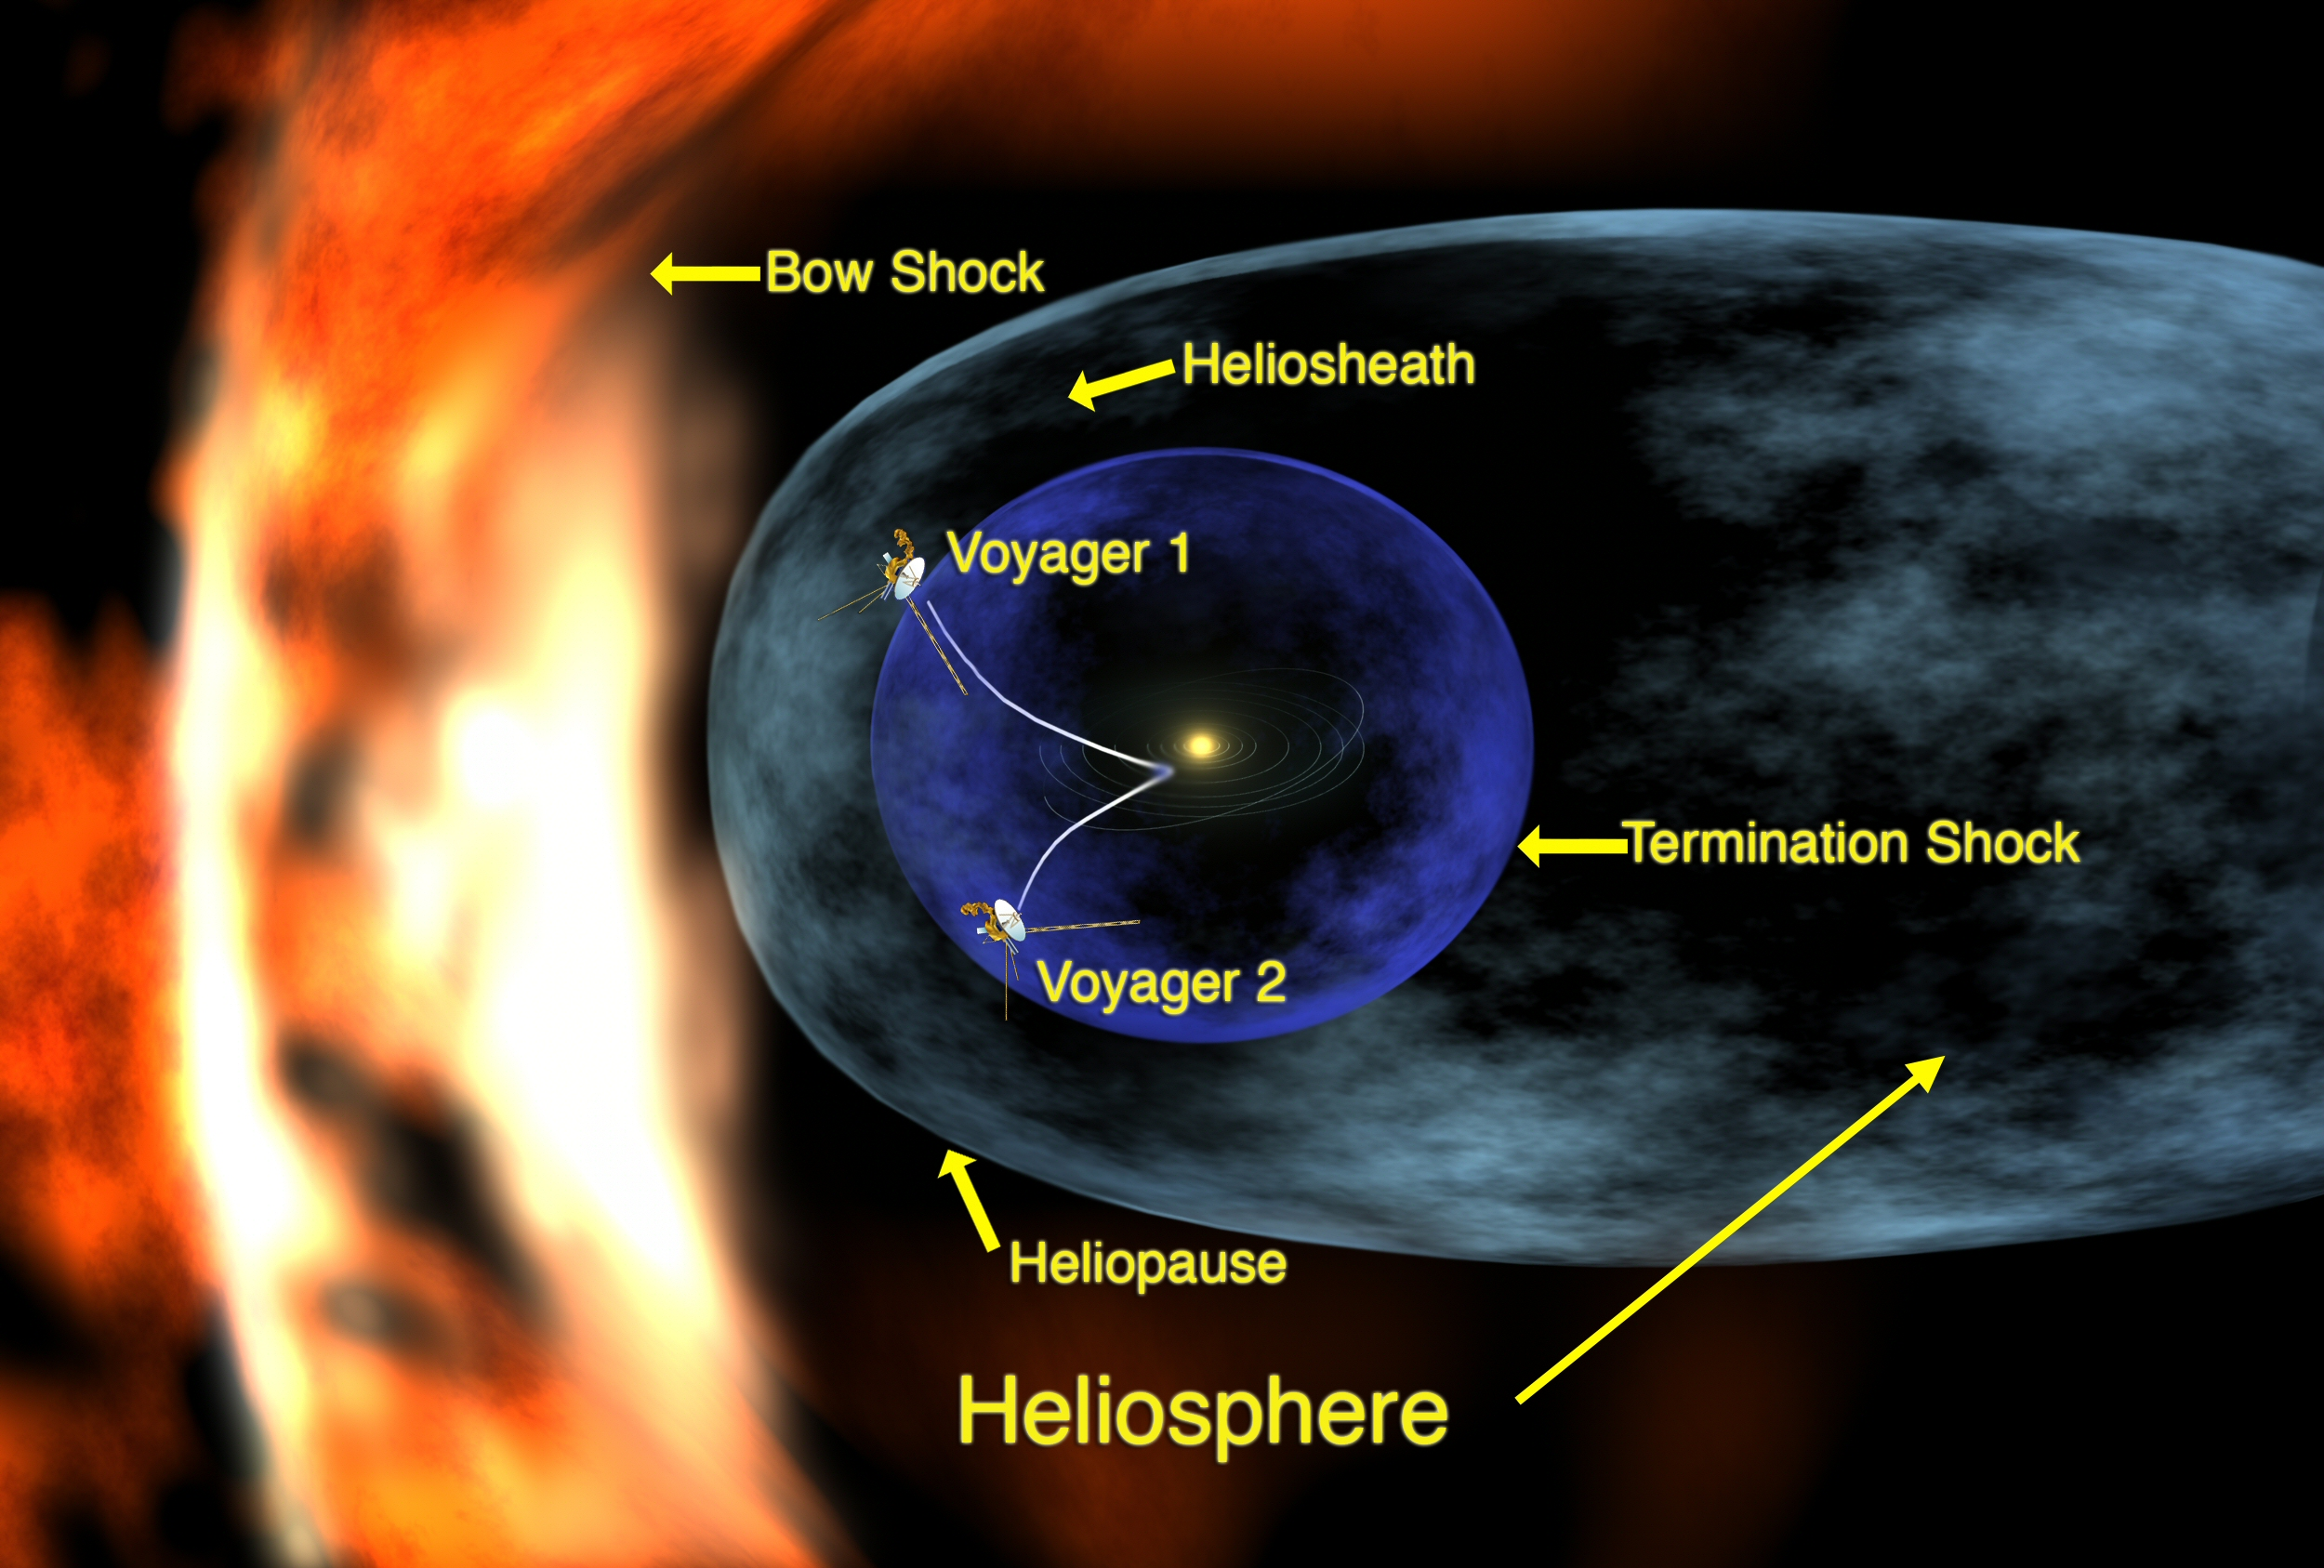
\includegraphics[width=0.43\textwidth,height=!]{./A/Voyager_1_entering_heliosheath_region.jpg}
\end{wrapfigure}  \vspace{0.1cm} The Solar wind blows out a cavity inside the
local ionised cloud (LIC). The heliosphere is about 100~AU in
diameter, with $N_e \sim 1 \times (1/ (r/\mathrm{AU})^2)~$cm$^{-3}$,
and $T_e \sim 10^4$~K. Optical absorption lines in the LIC have
$W_\lambda \sim 200$~m\AA, $b \sim$1~km~s$^{-1}$, and correspond to a
singly ionised gas with $T_e \sim 7000$~K, $N_e \sim 0.1$~cm$^{-3}$. 

\medskip

The LIC is embedded in the Local Bubble, $N_e \sim 5~10^{-3}$~cm$^{-3}$,
$T_e \sim 10^6~$K.

\medskip

Vallerga et al. (1993) show that the local ISM, the bulk of clouds
within the Local Bubble, is at rest in the LSR $\pm$11~km~s$^{-1}$ as
traced by CaII, and $\pm$3.6~km~s$^{-1}$ as traced by Na I. The solar
motion relative to the LSR is about 20~km~s$^{-1}$ in the direction of
Scorpius. 

\end{frame}

%\end{itemize}


\frame{\frametitle{Crude measures of the very local ISM density}



\begin{center}
%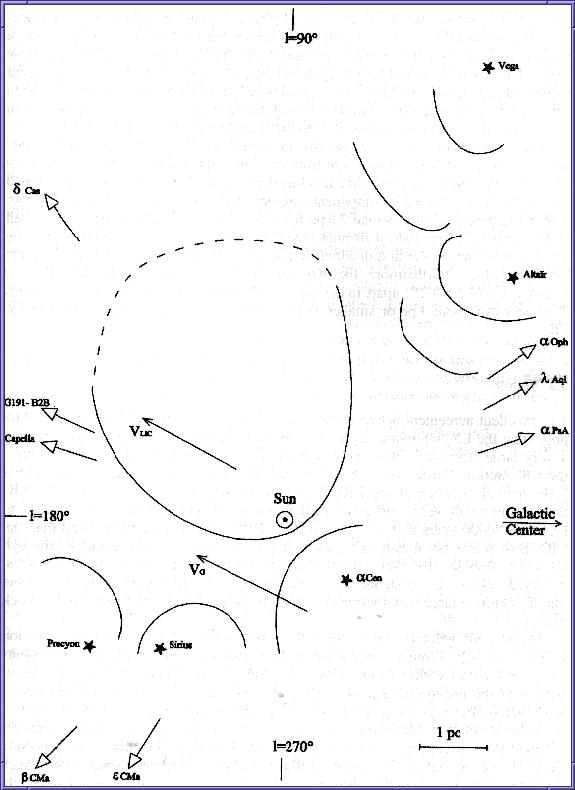
\includegraphics[width=!,height=0.7\figheight]{./A/localism_ferlet.jpg}
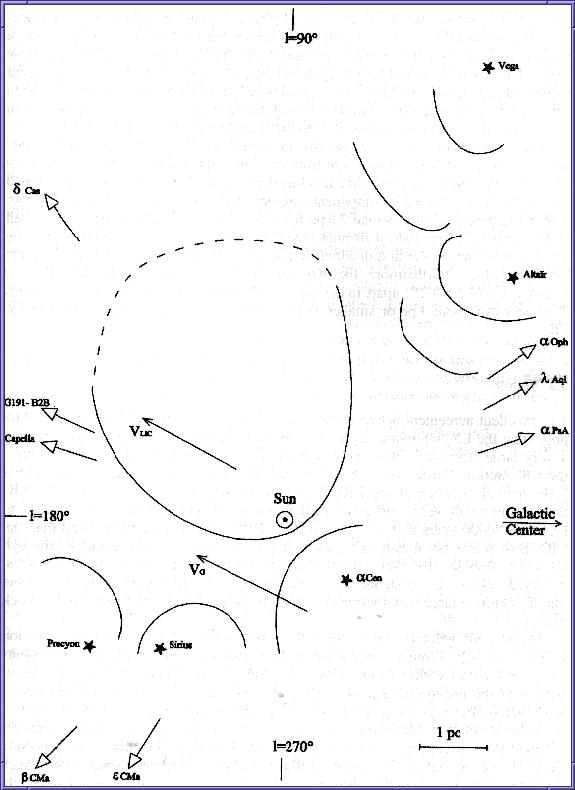
\includegraphics[width=!,height=\figheightscl]{./A/localism_ferlet.jpg}
%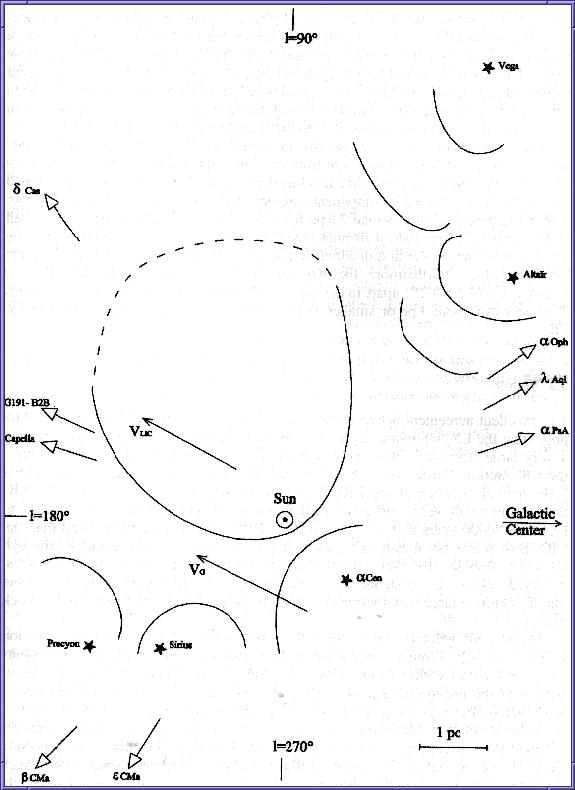
\includegraphics[width=!,height=1.0\figheight]{./A/localism_ferlet.jpg}
\end{center}
Ferlet (1999, A\&ARev, 9, 153). 


}

\subsection{The Local Bubble}

\frame{\frametitle{The Local Bubble.}

\begin{center}
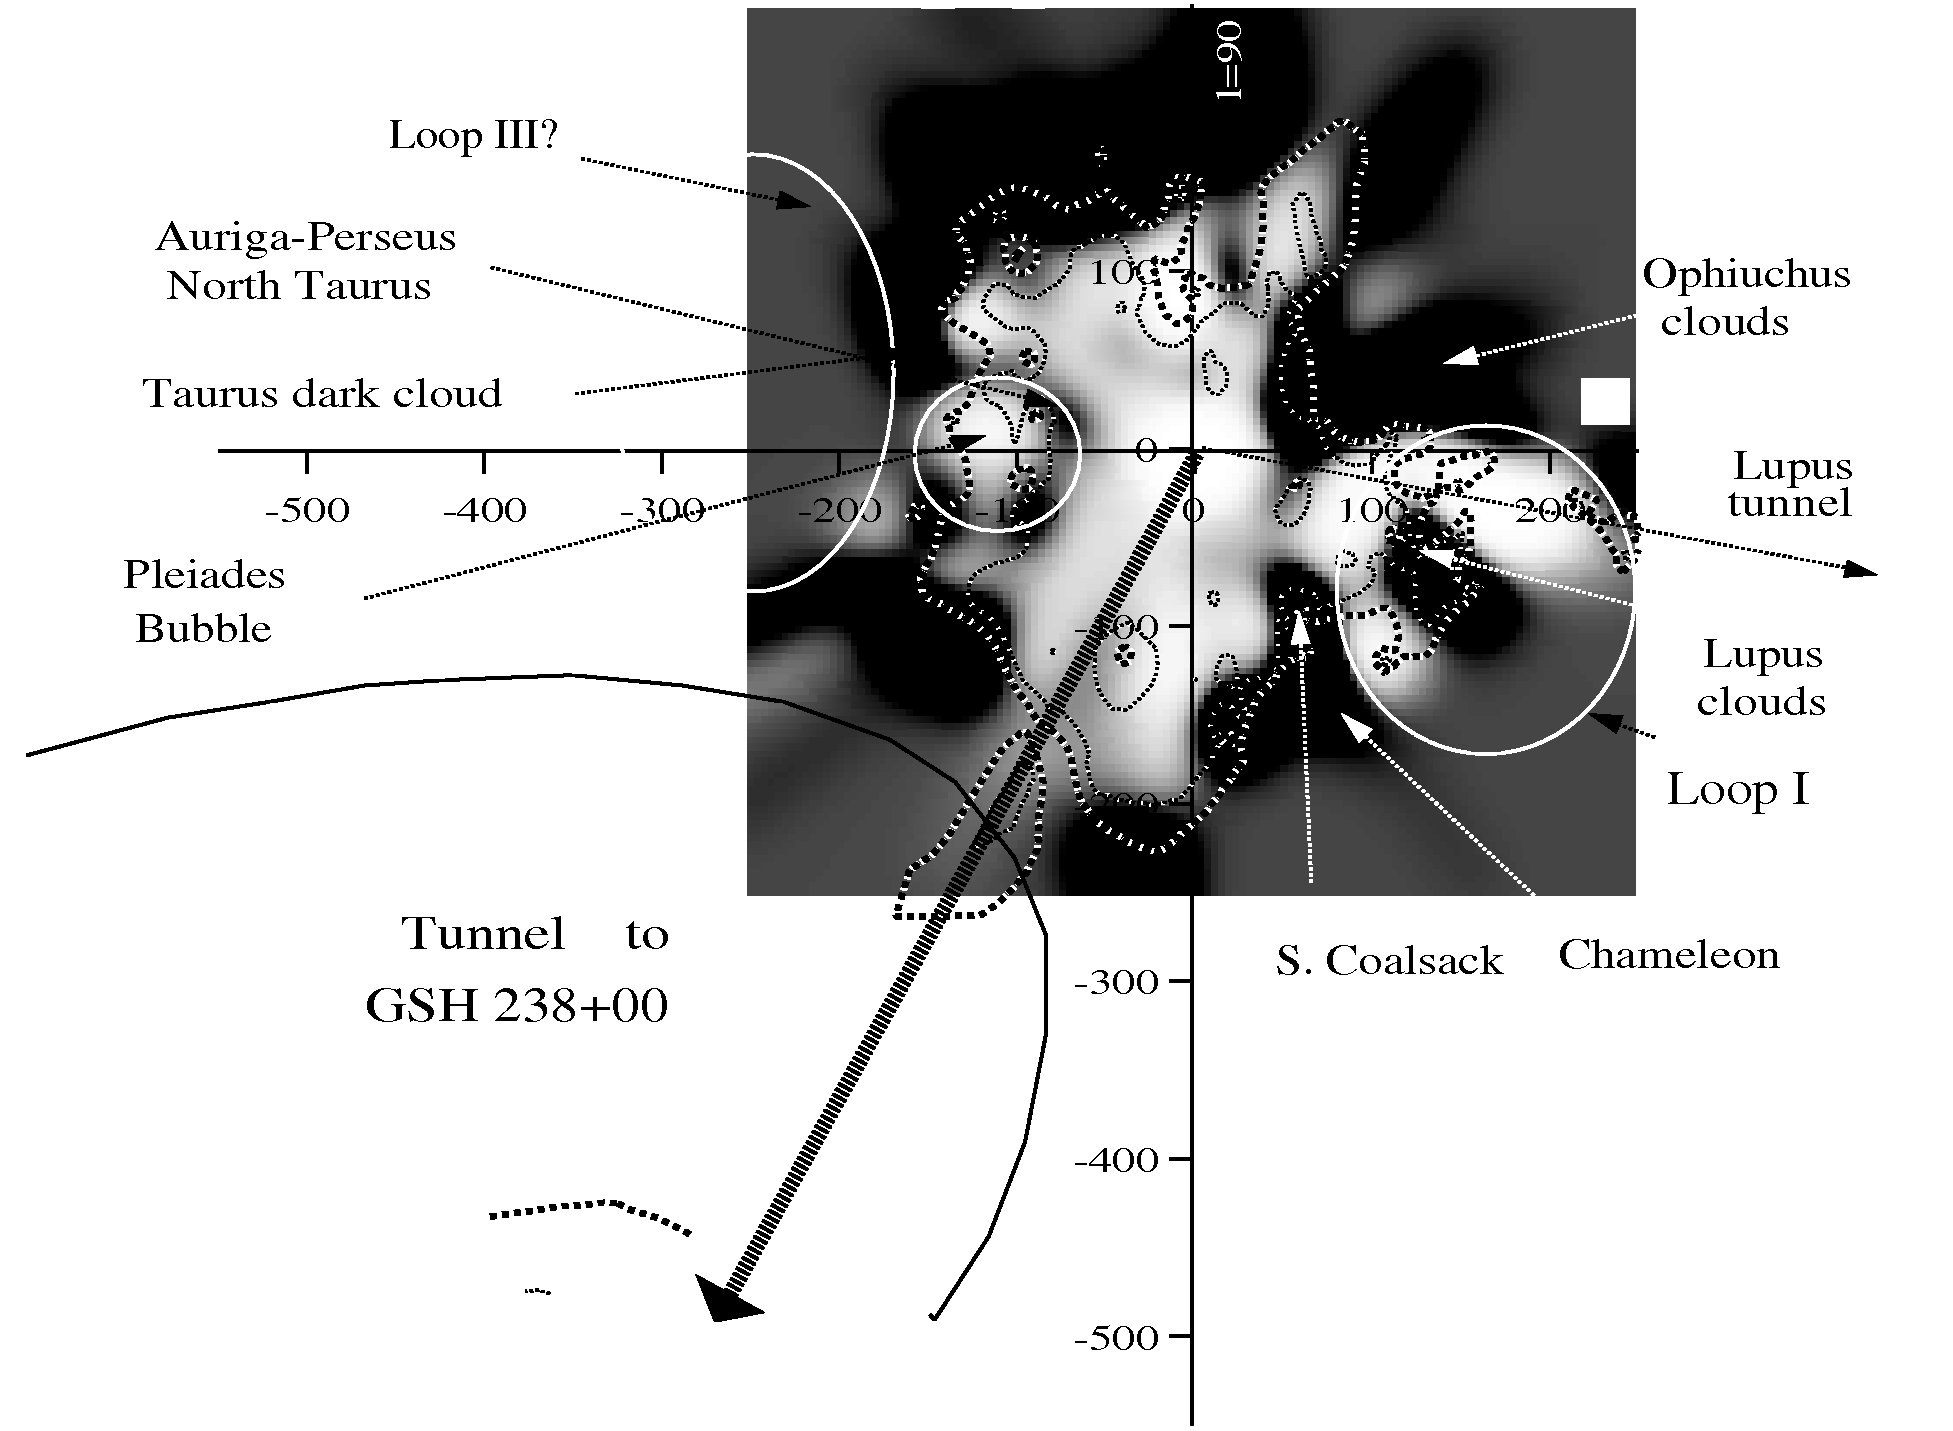
\includegraphics[width=0.9\textwidth,height=!]{./A/fig_lallement_fig1.jpg}
\end{center}
Na D lines maps. Contours at $W_\lambda =20~$m\AA~ and 50~m\AA~. Lallement et al. (2003, A\&A 411, 447).

}

\frame{\frametitle{The Local Chimney}

\vspace{-0.5cm}
\begin{minipage}[t]{0.5\textwidth}
\vspace{+0.5cm}
\begin{center}
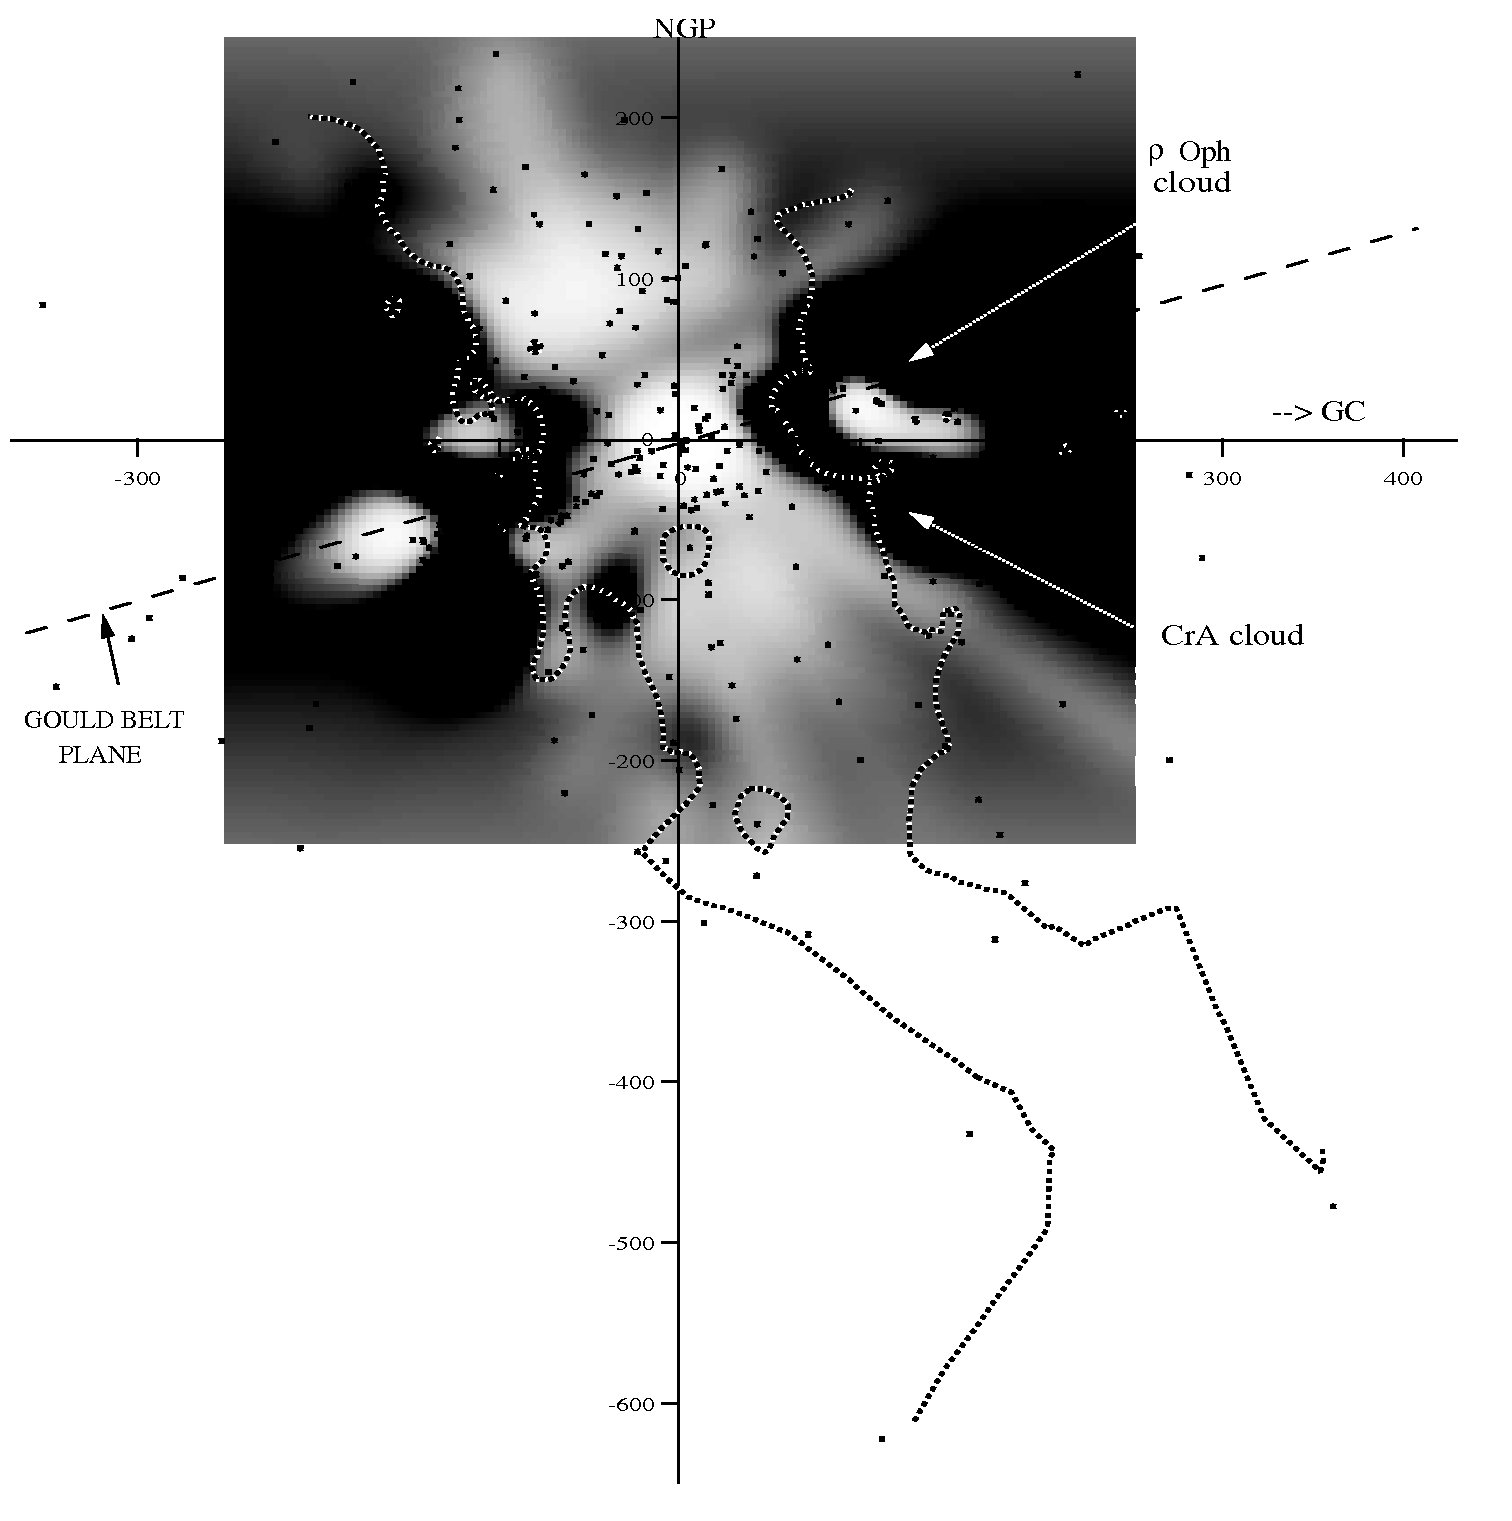
\includegraphics[width=\textwidth,height=!]{./A/fig_lallement_fig2.jpg}
\end{center}
\end{minipage}
\begin{minipage}[t]{0.5\textwidth}
\vspace{2cm}
\begin{itemize}
\item The Local Bubble appears to be squeezed into a Local Chimney by
SNR shells. The Local Chimney is very narrow: about 20~deg towards
each Galactic pole, corresponding to directions of minimal diffuse
H$\alpha$ and far-IR.
\end{itemize}
\end{minipage}


%\frame{\frametitle{The Local Chimney}
%
%%\vspace{-0.5cm}
%
%\begin{columns}[t,onlytextwidth]
%%\begin{columns}[t]
%
%\column{0.5\textwidth}
%
%\begin{center}
%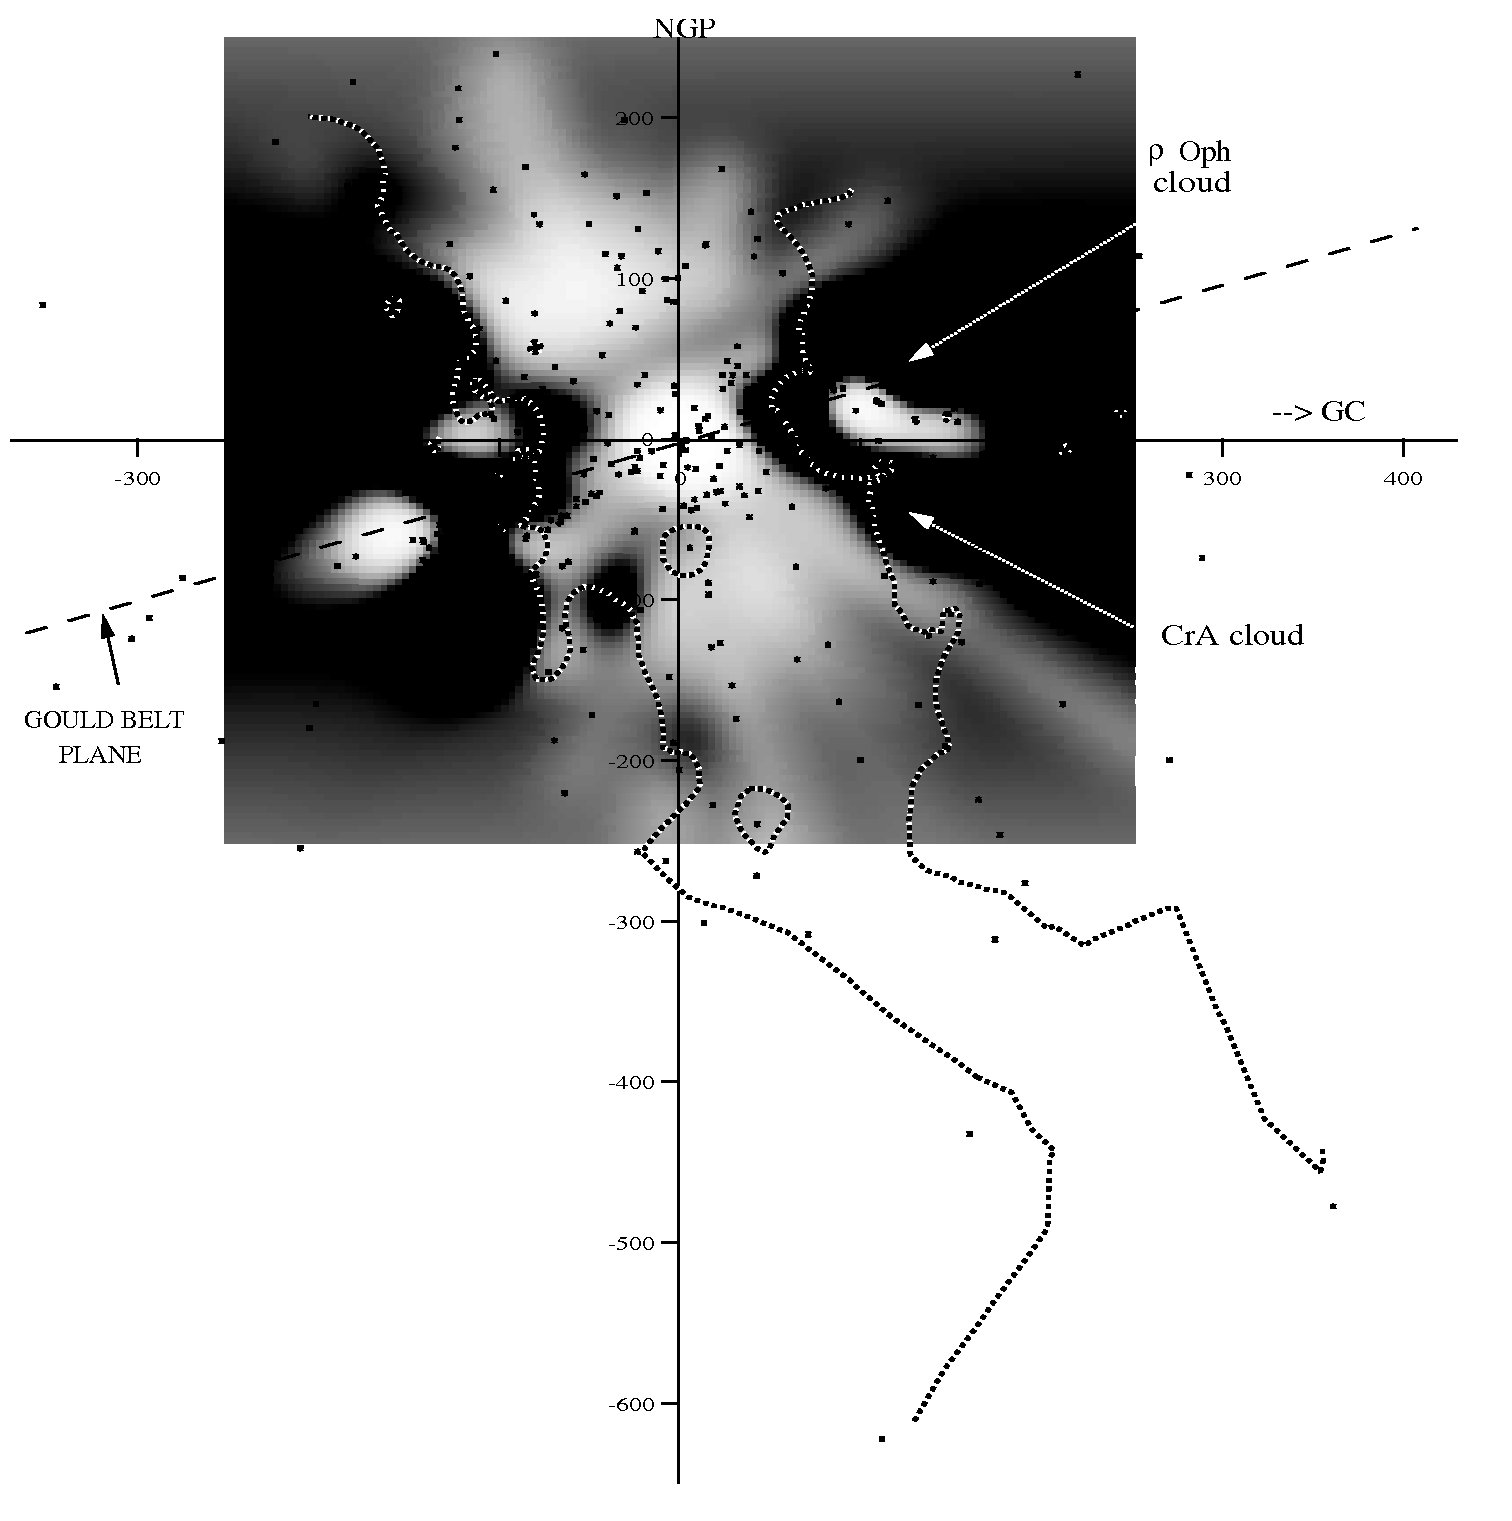
\includegraphics[width=\textwidth,height=!]{./A/fig_lallement_fig2.jpg}
%\end{center}
%
%\column{0.5\textwidth}
%
%The Local Bubble appears to be squeezed into a Local Chimney by
%SNR shells. The Local Chimney is very narrow: about 20~deg towards
%each Galactic pole, corresponding to directions of minimal diffuse
%H$\alpha$ and far-IR.
%\end{columns}
%
%
%}

\frame{\frametitle{Extragalactic windows}

Lallement et al. (2003) explain that ``no distinct and continuous
neutral boundary to the ends of the Local Chimney has been found in
either galactic hemisphere for distances $<$400~pc''. Crawford et
al. (2002) favor a picture of the inner galactic halo in which a
population of infalling IVCs lie along the Local Chimney. 

\medskip

{\large $\rightarrow$ The main absorbers in the local ISM towards
extragalactic objects are probably the boundaries of the Local
Chimney.}
}



\frame{\frametitle{Further 3D maps of the local ISM: face-on}
New density fields from Welsh, Lallement et al., 2010, A\&A, 510, A54


\begin{columns}[t,onlytextwidth]
\column{0.5\textwidth}

  \begin{center}
    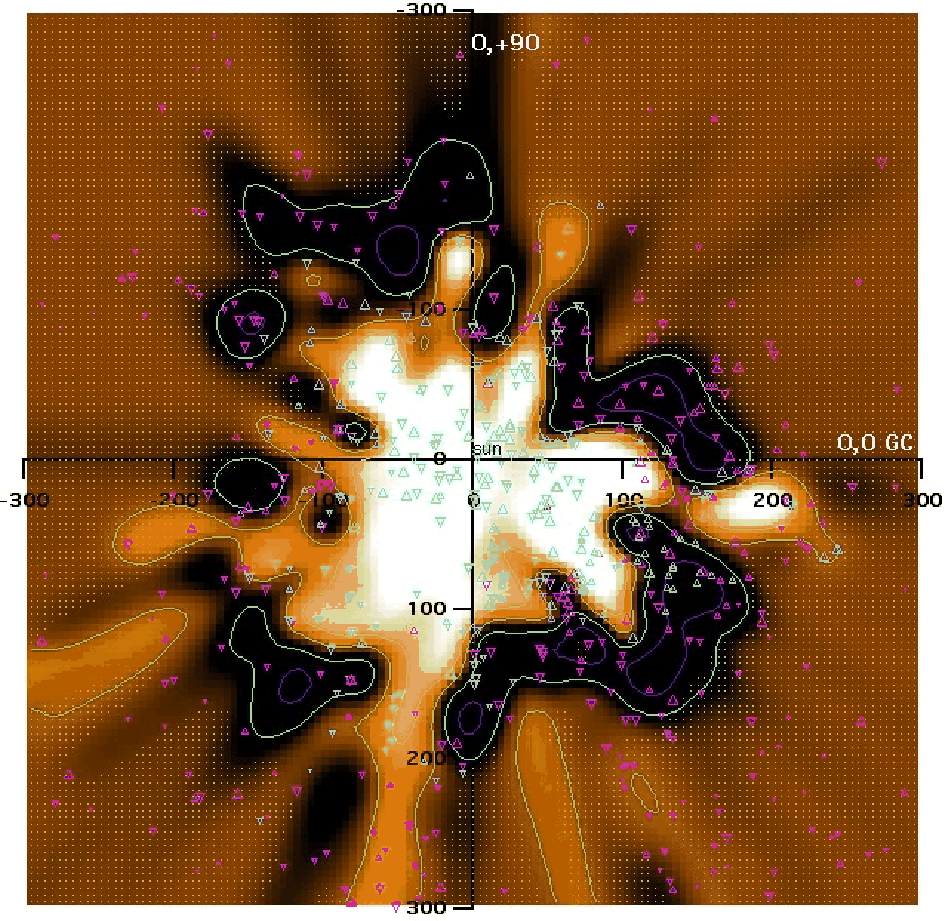
\includegraphics[width=\textwidth,height=!]{./A/welsh_fig12.png}

Na\,{\sc i} 
  \end{center}

\column{0.5\textwidth}


  \begin{center}
    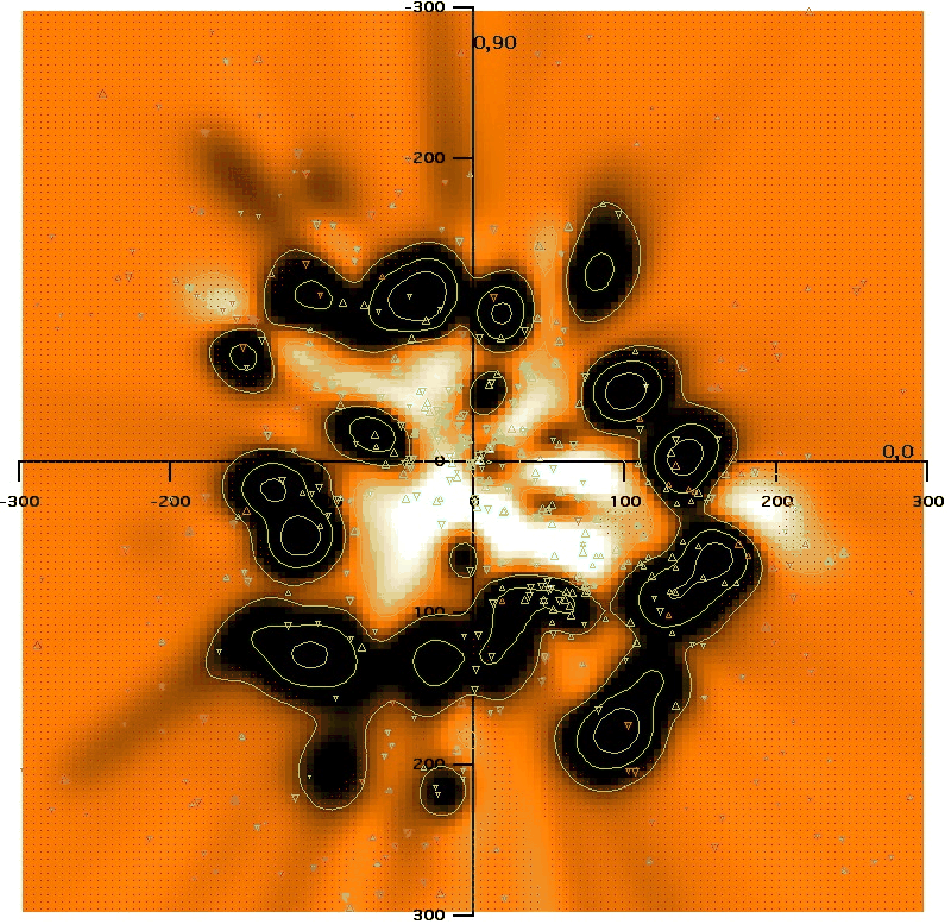
\includegraphics[width=\textwidth,height=!]{./A/welsh_fig15.png}

Ca\,{\sc ii}
  \end{center}
\end{columns}

}


\frame{ \frametitle{Further 3D maps of the local ISM: side view} 
\begin{columns}[t,onlytextwidth]
\column{0.5\textwidth}
  \begin{center}
    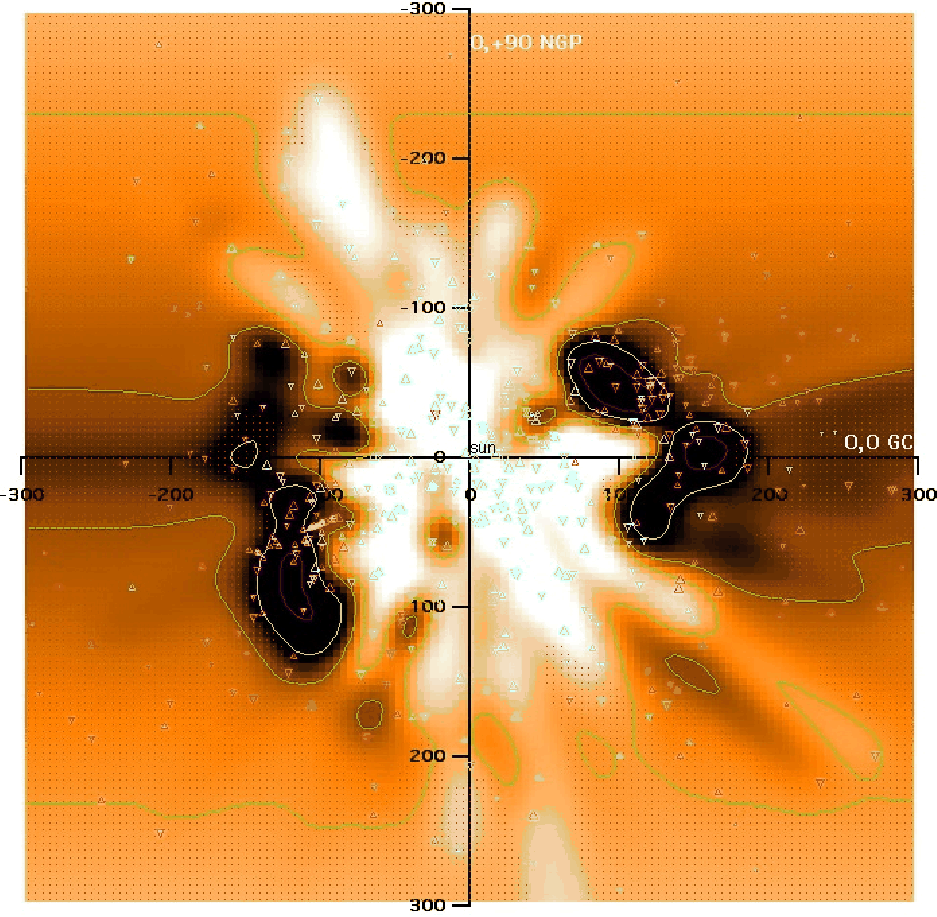
\includegraphics[width=\textwidth,height=!]{./A/welsh_fig13.png}

Na\,{\sc i} 
  \end{center}

\column{0.5\textwidth}
  \begin{center}
    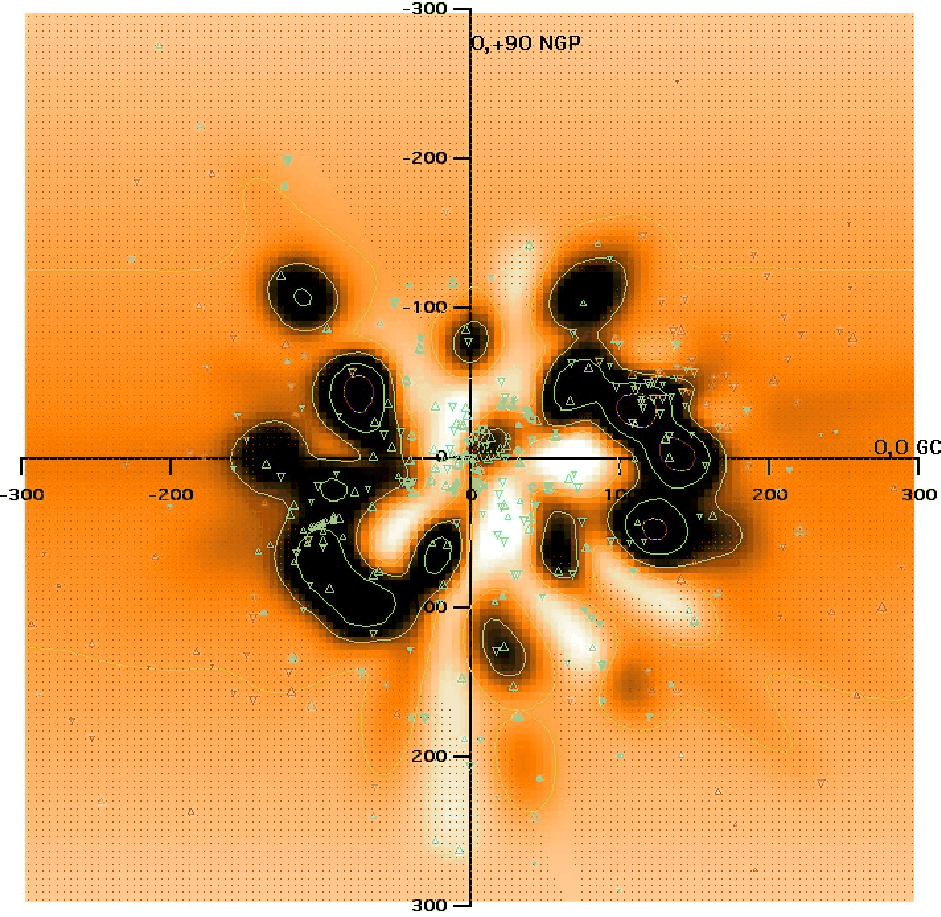
\includegraphics[width=\textwidth,height=!]{./A/welsh_fig16.png}

Ca\,{\sc ii}
  \end{center}
\end{columns}

}







\section{Morphology of interstellar clouds}

\subsection{Old model for clouds in thermal equilibrium}

\frame{\frametitle{Morphology of interstellar clouds}
%\hypersetup{pdfpagetransition=Dissolve}





Interstellar absorption lines (e.g.: CH$^{+}\lambda 4232$\AA,
CH$\lambda 4300$\AA, CN$\lambda 3875$\AA, etc..., ref: Dunham 1937,
PASP, 49, 26; Douglas \& Herzberg 1941, ApJ, 94, 381; Adams 1949,
ApJ, 109, 354) 

%\begin{minipage}[t]{11cm}
%\begin{center}
%\includegraphics[width=11cm,height=!]{fig_ZOPH.pdf}
%\end{center}
%\end{minipage}
%\hfill
%\begin{minipage}[t]{11cm}


%\footnote{S/N~2000, $\Delta~\lambda$~0.05\AA,
%(Casassus et al. 2004, in prep)}


\begin{center}
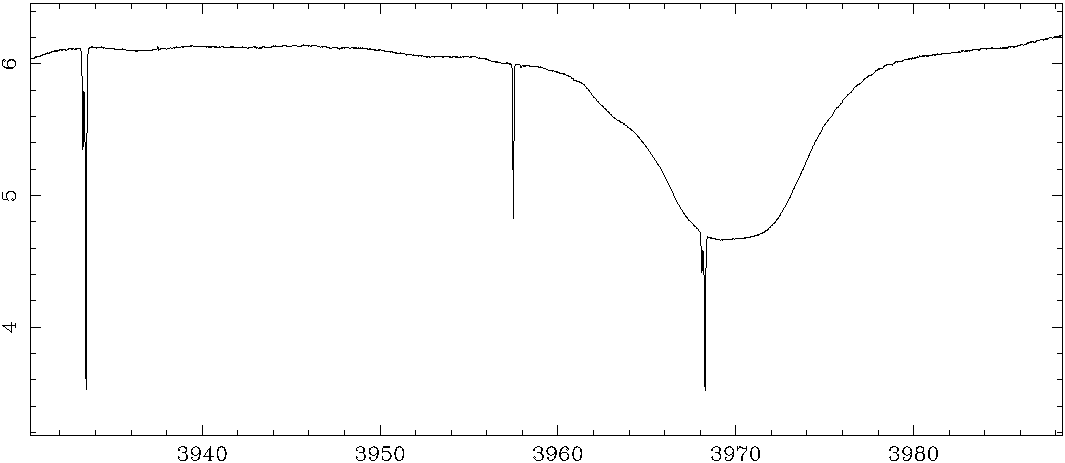
\includegraphics[width=0.7\textwidth,height=!]{./A/zetaOph_3960.pdf}\\
\mbox{$\zeta$Oph VLT+UVES spectrum around $\sim$3960\AA}
\end{center}


}


\frame{ \frametitle{Old model} 
\begin{center}
$\zeta$Oph VLT+UVES spectrum around  $\sim$3960\AA - zoom.
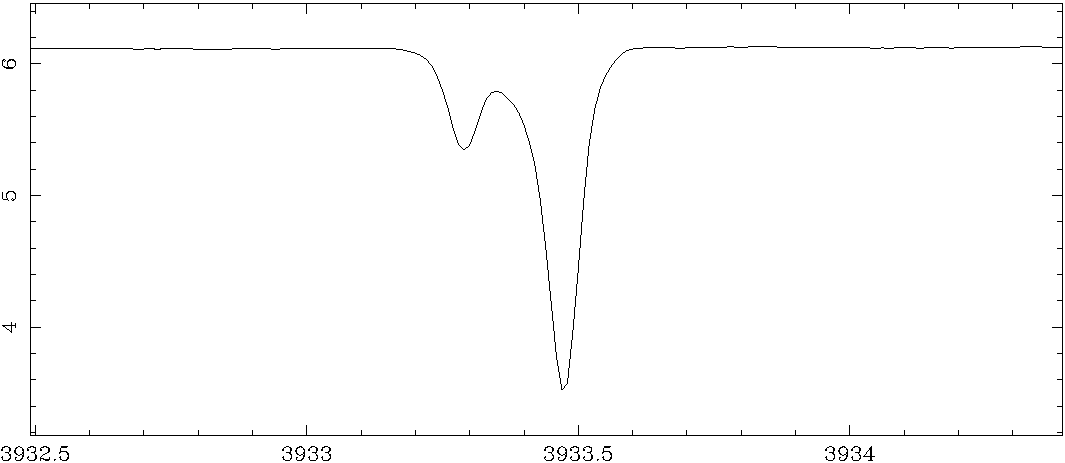
\includegraphics[width=0.7\textwidth,height=!]{./A/zetaOph_CaII3933.pdf}
\end{center}

$\rightarrow$ \\ model of discrete clouds confined
by pressure equilibrium with the the intercloud medium, $T\sim10^6$K
(e.g. Spitzer, 1956, ApJ, 124, 20), confirmed through the observation
of O{\sc~vi}$\lambda$1031 absorption towards nearby stars ({\em
Copernicus}$\sim$1973, {\em FUSE} $\sim$2002).

}

\subsection{Realistic descriptions}

\frame{ \frametitle{Problems with the discrete cloud model}

(Elmegreen \& Falgarone, 1996, ApJ, 471, 816)
\begin{itemize}
\item Supersonic motions imply that the dynamics of the clouds are
dominated by shocks, not thermal pressure.
\item Improving the angular resolution of interstellar cloud maps
invariably result in the discovery of substructure.
\item Linear size, mass, and velocity dispersion are related by power
laws, which can be characterised through scaling laws: \( N(L) \propto
M(L) \propto L^{D}.  \) Power laws are typical of self-similar
structures. A function  $y=f(x)$ whose properties only change by a
factor $b$ when applying a scaling factor $a \times x$ must fulfill 
\( f(a\,x) = b f(x) \). Scaling $k$ times,   $x = a^k x_\circ $, and $y =
b^k y_\circ$, from which $y = x^c$, with $c = \ln(b)/\ln(a)$. If $y$
is the number of structures or the mass, and if $x$ is size, then $c$
is the fractal dimension of the selfsimilar structure. 

\end{itemize}

\vfill

}
\begin{frame} \frametitle{Morphology of the  ISM: scaling laws} 

\begin{center}
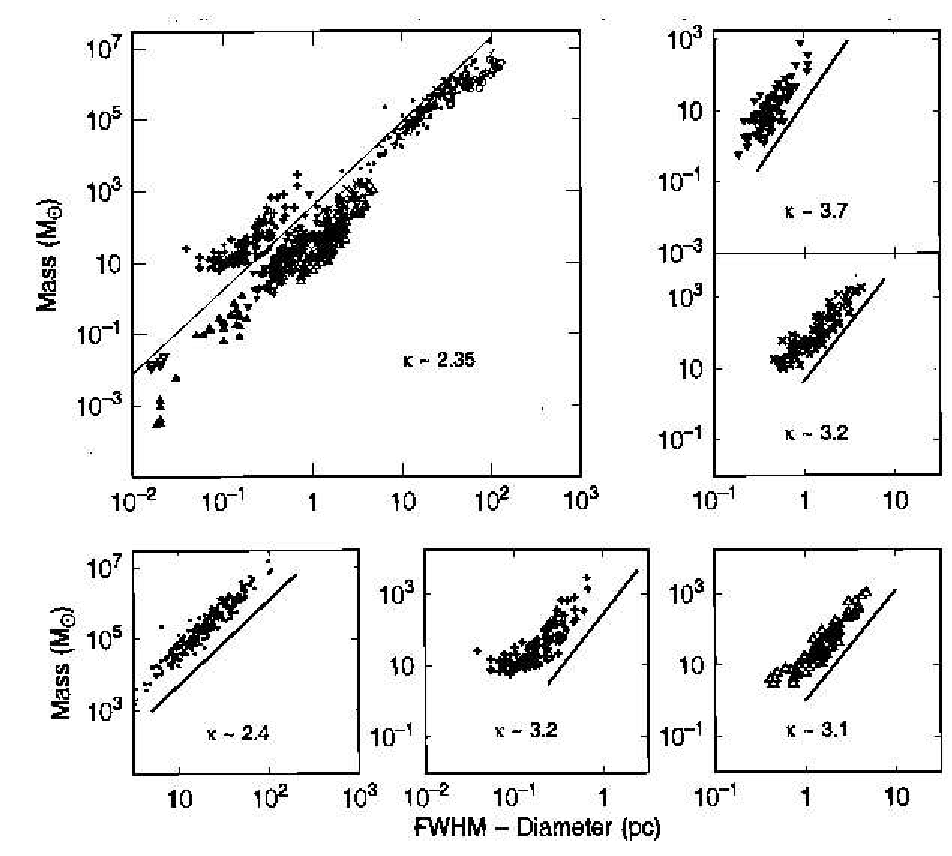
\includegraphics[width=\textwidth,height=!]{./A/ml.pdf}
\end{center}



\end{frame}

\begin{frame}{Morphology of the ISM: Armonic analysis} 

The structure of the ISM can also be described by an armonic analysis,
with the power spectrum of the specific intensity maps: \( P(k)
\propto k^{\alpha} \), in which  $P(k)$ is the modulus of  \( F(k) = \int
dxdy I(x,y) \exp(2i\pi
\vec{k}.\vec{x}), \) with an angle average for isotropic
distributions. The power spectrum allows the inference of basic
properties of the emission maps, such as characteristic angular sizes,
relative importance of angular scales, etc....  \\

For scales larger than $>$10~deg, it is necessary to take into account
the curvature of the celestial sphere:
\[I(\hat{r},\nu) = \sum_l\sum_m Y_{lm}(\hat{r}) a_{lm}(\nu),
\] and the power spectrum is 
\(
C_l \equiv 1/(2l+1) \sum_{m=-l}^{m=+l} \langle
\|a_{lm}(\nu)\|^2 \rangle 
\), in the definition by  Tegmark \& Efstathiou, 1996, MNRAS, 281,
1297.  In a flat aproximation to the celestial sphere, $k =
(l+1/2)/2\pi$, and $k^2P(k) = l (l+1) C_l / (2\pi)^2$, with $k$ in
rad$^{-1}$.

\end{frame}

\frame{\frametitle{Example power spectra} 

\begin{itemize}
\item CMB. 
\item white noise, with  $P(k) = $~Cte.  Example: point sources with a
random distribution (i.e. Poisson). On average,
\(
\langle a_{lm} \rangle = \int d\Omega  ~Y^{\star}_{lm}(\Omega) \langle
  I(\hat{r})\rangle,
\) with  $\langle I(\hat{r})\rangle = \frac{N}{4\pi} \phi$, where $\phi$ 
  is the average flux density of $N$ sources in the sky. $\langle n
  \rangle = N/4\pi$ follows a Poisson distribution: $\langle n^2
  \rangle - \langle n \rangle^2 = \langle n \rangle$.
\(
\langle \| a_{lm} \|^2 \rangle = \int d\Omega d\Omega^\prime
 ~  Y^{\star}_{lm}(\Omega)  Y_{lm}(\Omega^\prime) ~ \langle
  I(\Omega)  I(\Omega^\prime)) \rangle,
\)\\ and as   \( \langle
  I(\Omega)  I(\Omega^\prime) \rangle = \delta(\Omega-\Omega^\prime)
  \phi^2 \langle n \rangle\)  \( \Rightarrow C_l = \phi^2 \langle n
  \rangle.\)  



\item power spectrum of the  {\em IRAS} syrvey. 
Ref: Gautier et al. (1992, AJ, 102, 1313), Miville-Desch\^eches et
al. (2007, A\&A, 469, 595):
$P(k) \propto k^{-2.9}$.
\item Recent analysis by  Oliveira-Costa et al. (2002, ApJ, 567,
  363). 
\end{itemize}

\vfill


}
\frame{\frametitle{ISM power spectra}  


\begin{center}
  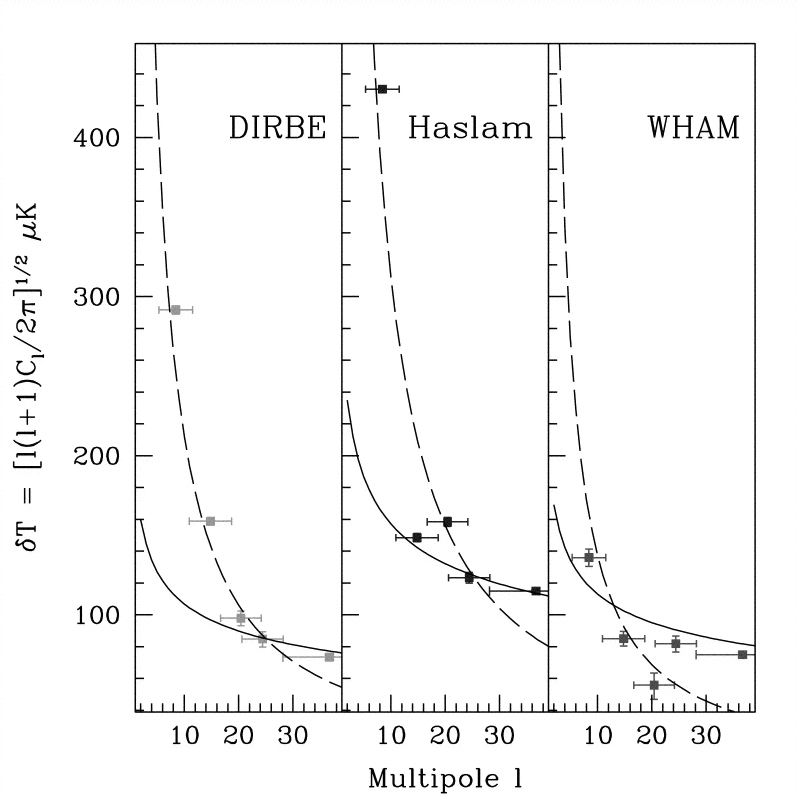
\includegraphics[width=!,height=\figheightscl]{./A/fg2.png}
  %{\tiny From \href{http://klab.agsci.colostate.edu/aegypti/aegypti.html}
  %{http://klab.agsci.colostate.edu/aegypti/aegypti.html}}
\end{center}

\vfill

}

\frame{ \frametitle{Morphology of the ISM: armonic analysis} 


\begin{columns}[t,onlytextwidth]

\column{0.5\textwidth}

  \begin{center}
    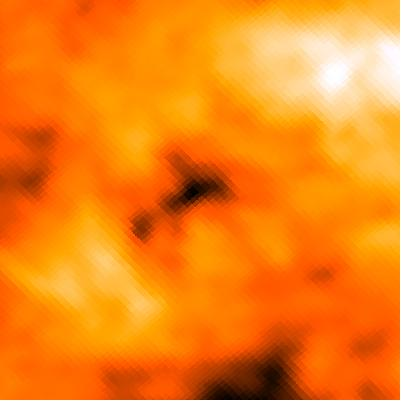
\includegraphics[width=\textwidth,height=!]{./A/zoph_sfd_3deg.jpg}
  \end{center}


\column{0.5\textwidth}

  \begin{center}
    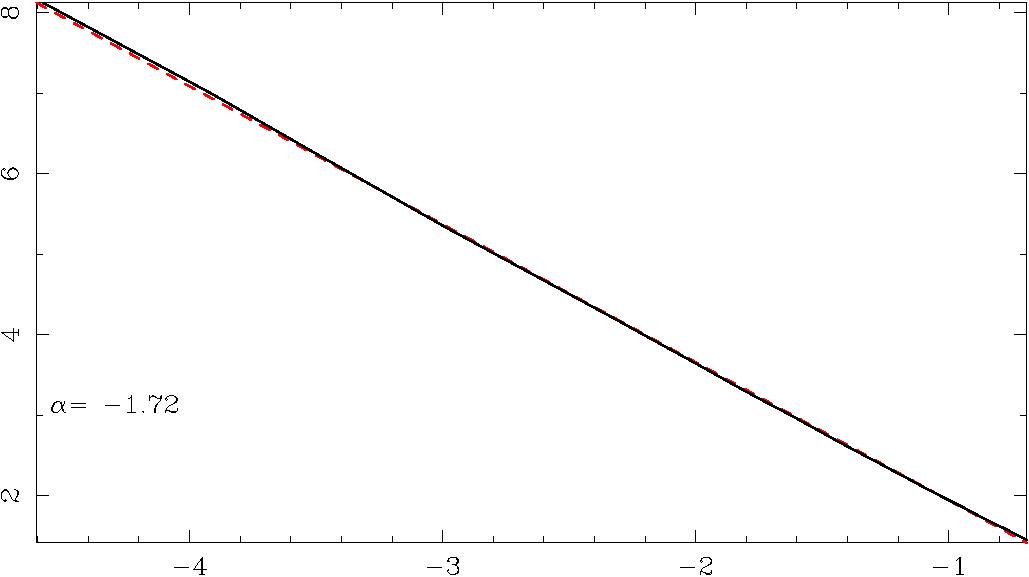
\includegraphics[width=\textwidth,height=!]{./A/sfdpowerspec.pdf}
  \end{center}

\end{columns}


\vfill

}

\frame{ \frametitle{Morphology of the ISM: relationship   between scaling laws and the power spectrum}

A self similar structure with a self-similar exponent $H$ has a 1-D
power spectrum $P(k) = \mathrm{Cte}~ k^{-1-2\,H}$ (e.g.  ``Fractals, a
User's Guide for the Natural Sciences'', Hastin \& Sugihara, 1993,
Oxford Science Publications).  \\

\medskip

A recipe for simulating fractals is therefore to generate a
power-spectrum whose amplitude has a variance of $k^{-1-2\,H},$ and
with random phases. Passing to the celestial plane and taking real
parts, one gets a self-similar structure with fractal dimension
$2\,H$, and with random phases. Switching to the image plane and
taking real parts one obtains a self-similar structure with fractal
dimension $2\,H$, and with random phases. The requisite $P(\hat{k}) =
P^{\star}(-\hat{k})$ generates a real map.

}

\frame{ \frametitle{Morphology of the ISM: examples} 

Fractal analysis of an H\,{\sc i}~21~cm in the LMC (Elmegreen, Kim,
Staveley-Smith ,2001,ApJ,548,749)x.

\begin{center}
  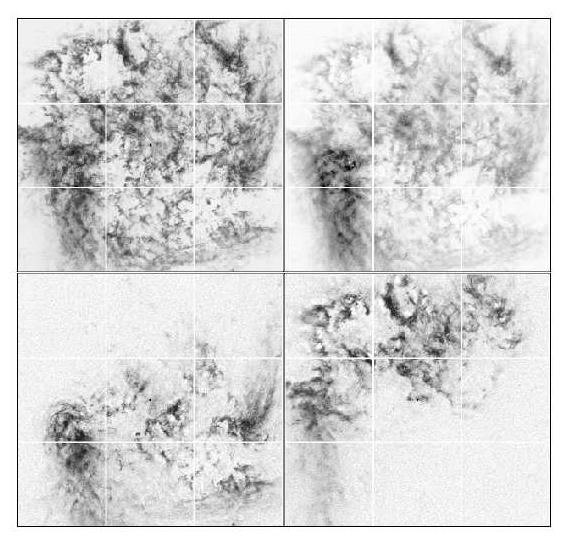
\includegraphics[width=0.7\textwidth,height=!]{./A/elemegreen_lmc_example_fig1_clip}
\end{center}

\vfill
}
\frame{ \frametitle{Morphology of the ISM: examples} 

\begin{columns}[t,onlytextwidth]

\column{0.5\textwidth}

  \begin{center}
    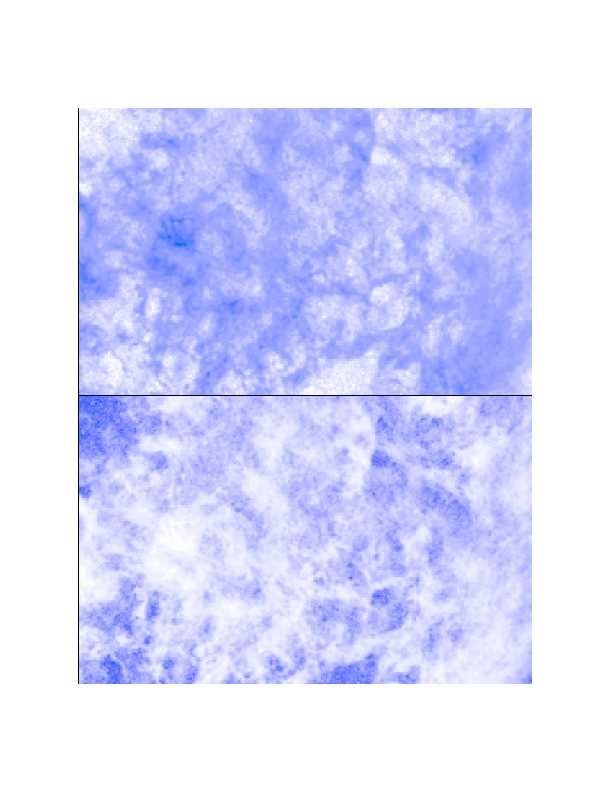
\includegraphics[width=\textwidth,height=!]{./A/elmegreen_lmc_example_fig10}
  \end{center}

\column{0.5\textwidth}

  \begin{center}
    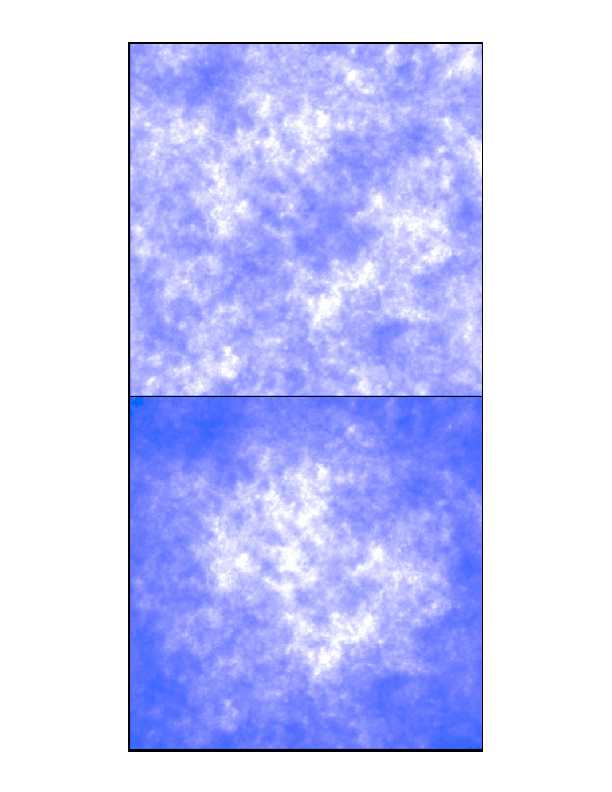
\includegraphics[width=\textwidth,height=!]{./A/elmegreen_lmc_example_fig15}
  \end{center}

\end{columns}

}

\section{Phases of the ISM}

\frame{\frametitle{Phases of the ISM} 

Molecular components (H$_2$), atomic (H\,{\sc i}, photo-dissociation
regions, or PDRs), ionised (H\,{\sc ii} regions, with T~10$^4$~K), and
hot plasma, with $T~10^6$~K.

\begin{center}
  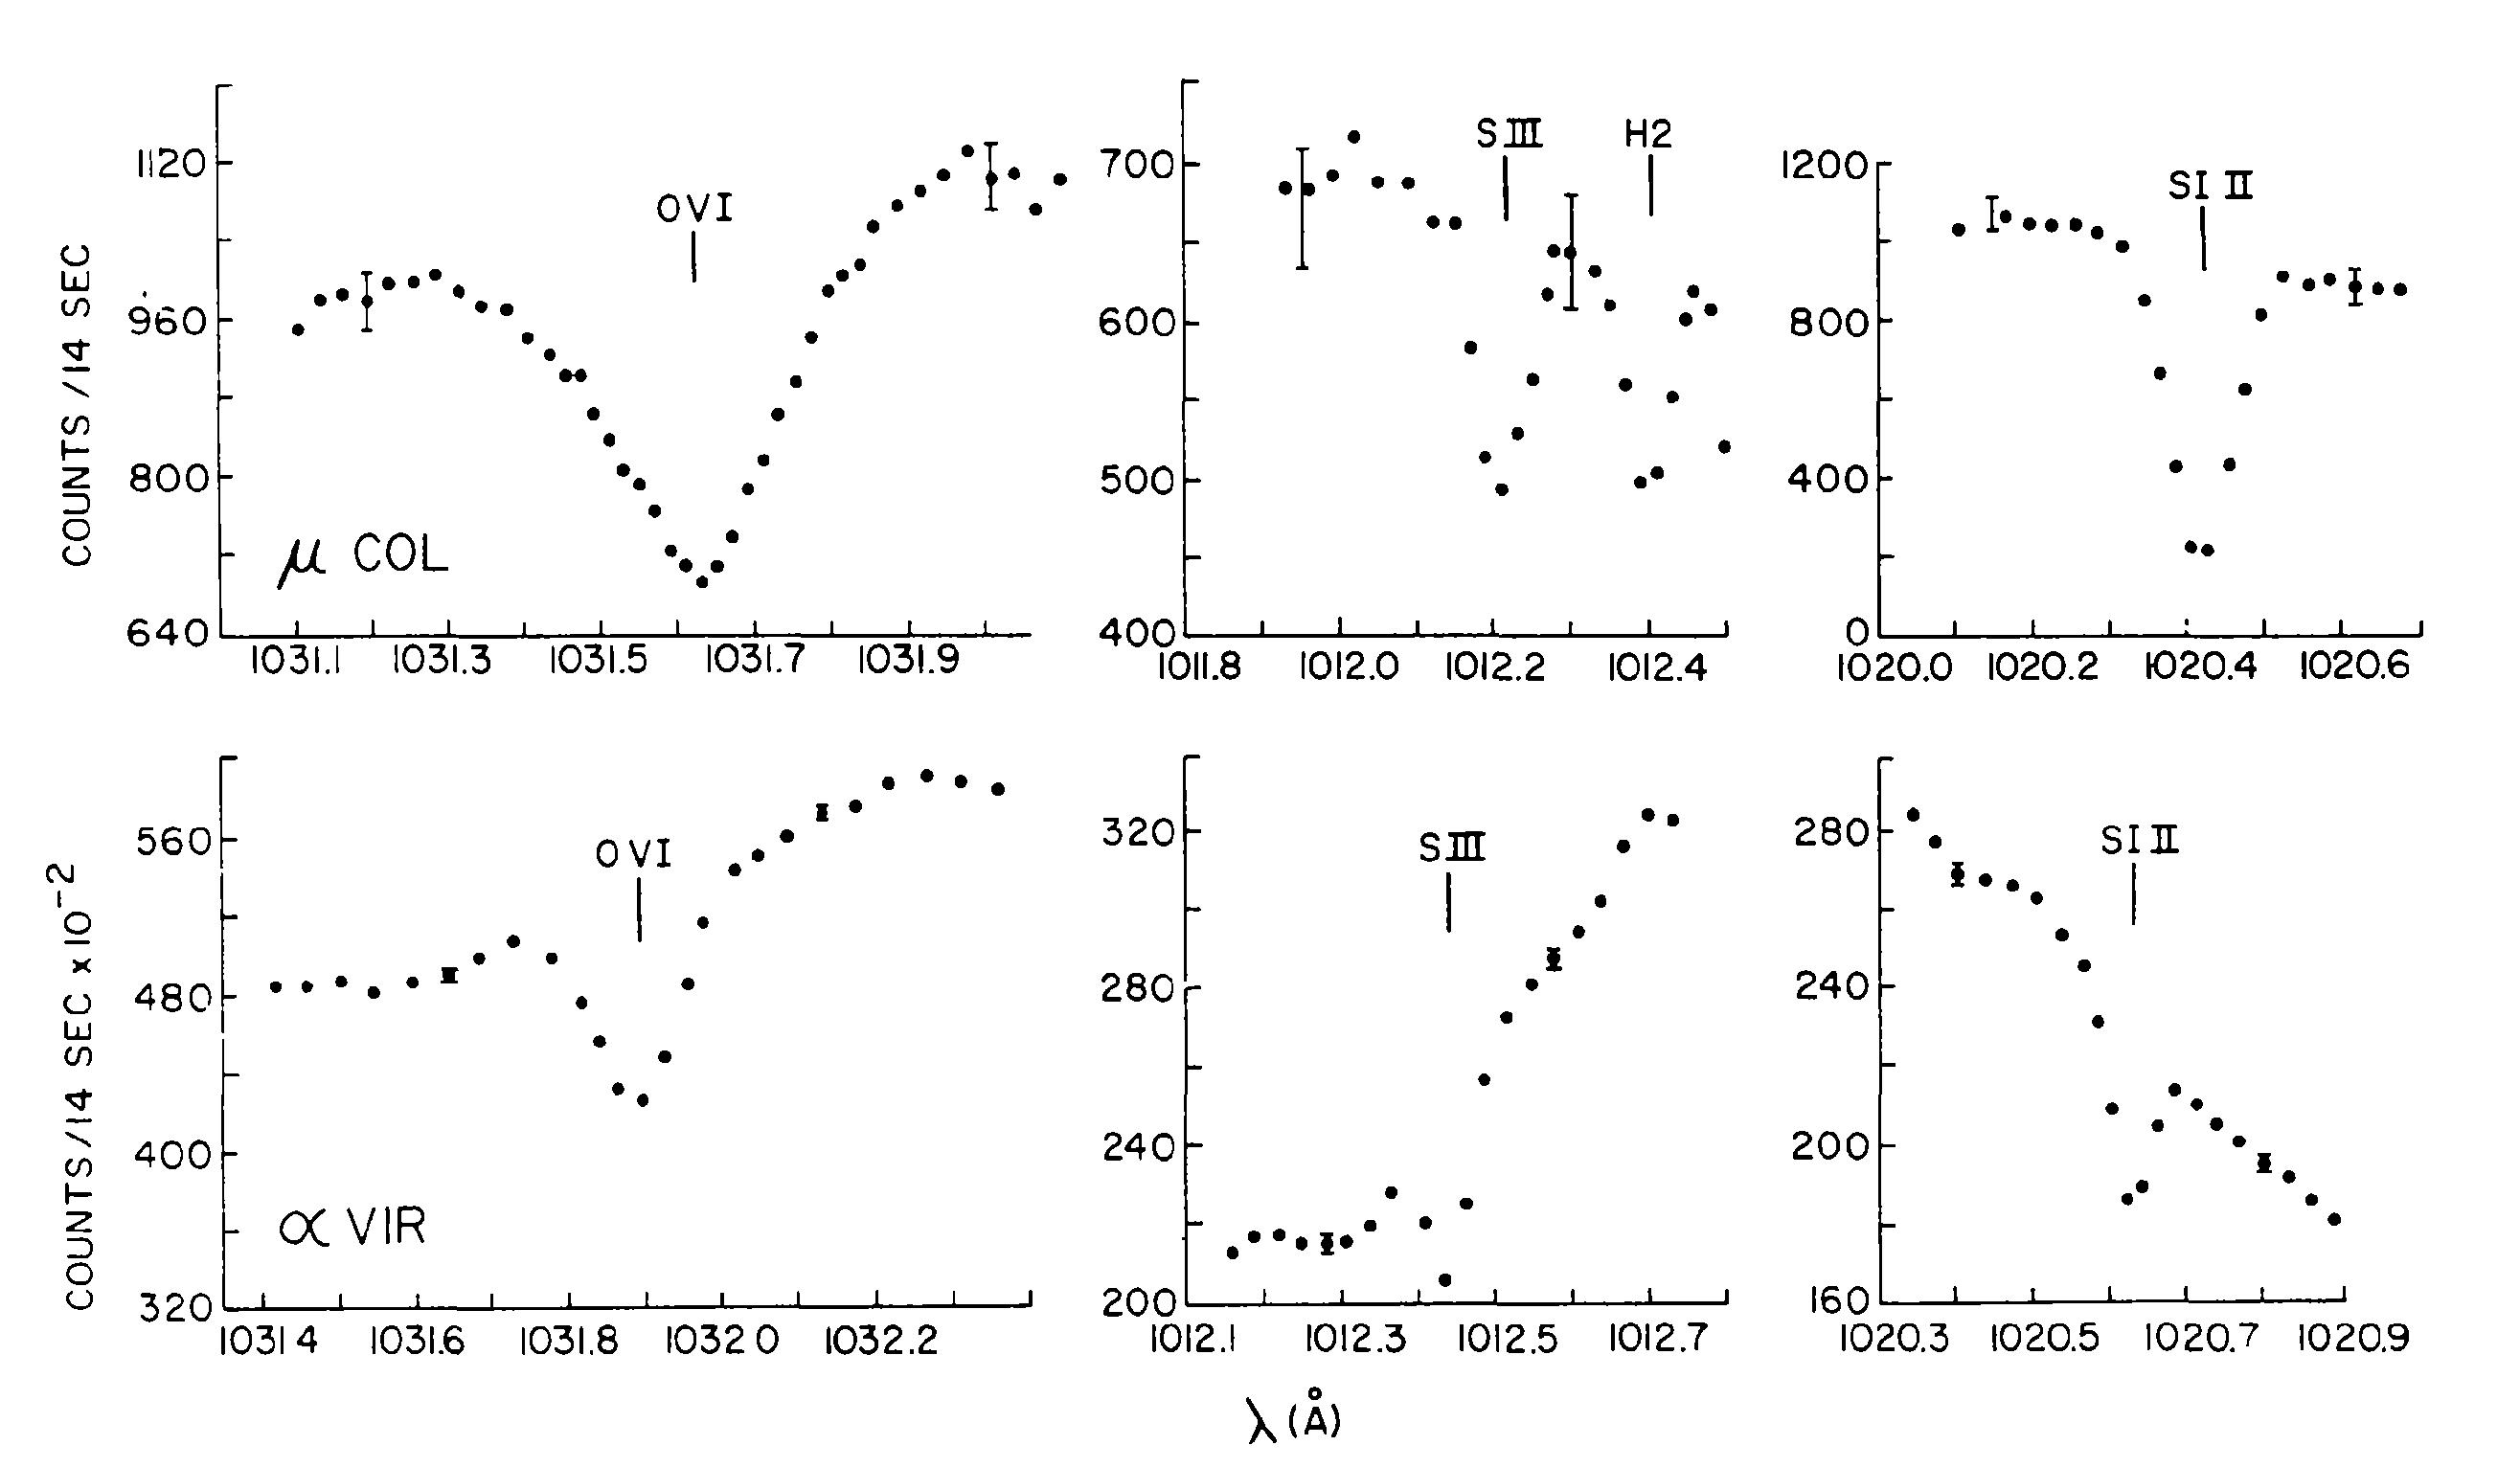
\includegraphics[width=\textwidth,height=!]{./A/york1974_ovi.jpg}
  %{\tiny From \href{http://klab.agsci.colostate.edu/aegypti/aegypti.html}
  %{http://klab.agsci.colostate.edu/aegypti/aegypti.html}}
\end{center}
\vfill

}

\frame{ \frametitle{Phases of the interstellar medium:
  dust in the H\,{\sc~i} region }


Depletion pattern in the neutral phase of the ISM towards  $\zeta$Oph
$\rightarrow$ dust at  18~K. 

\begin{columns}[t,onlytextwidth]


\column{0.5\textwidth}
\begin{center}
  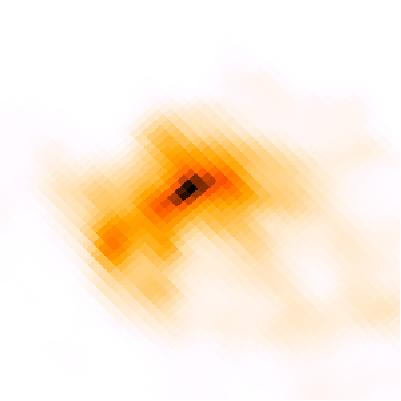
\includegraphics[width=\textwidth,height=!]{./A/zoph_sfd.jpg}
  {\tiny  {\tt http://skyview.gsfc.nasa.gov} }
\end{center}

\column{0.5\textwidth}
\begin{center}

% \rotatebox{-90}{ 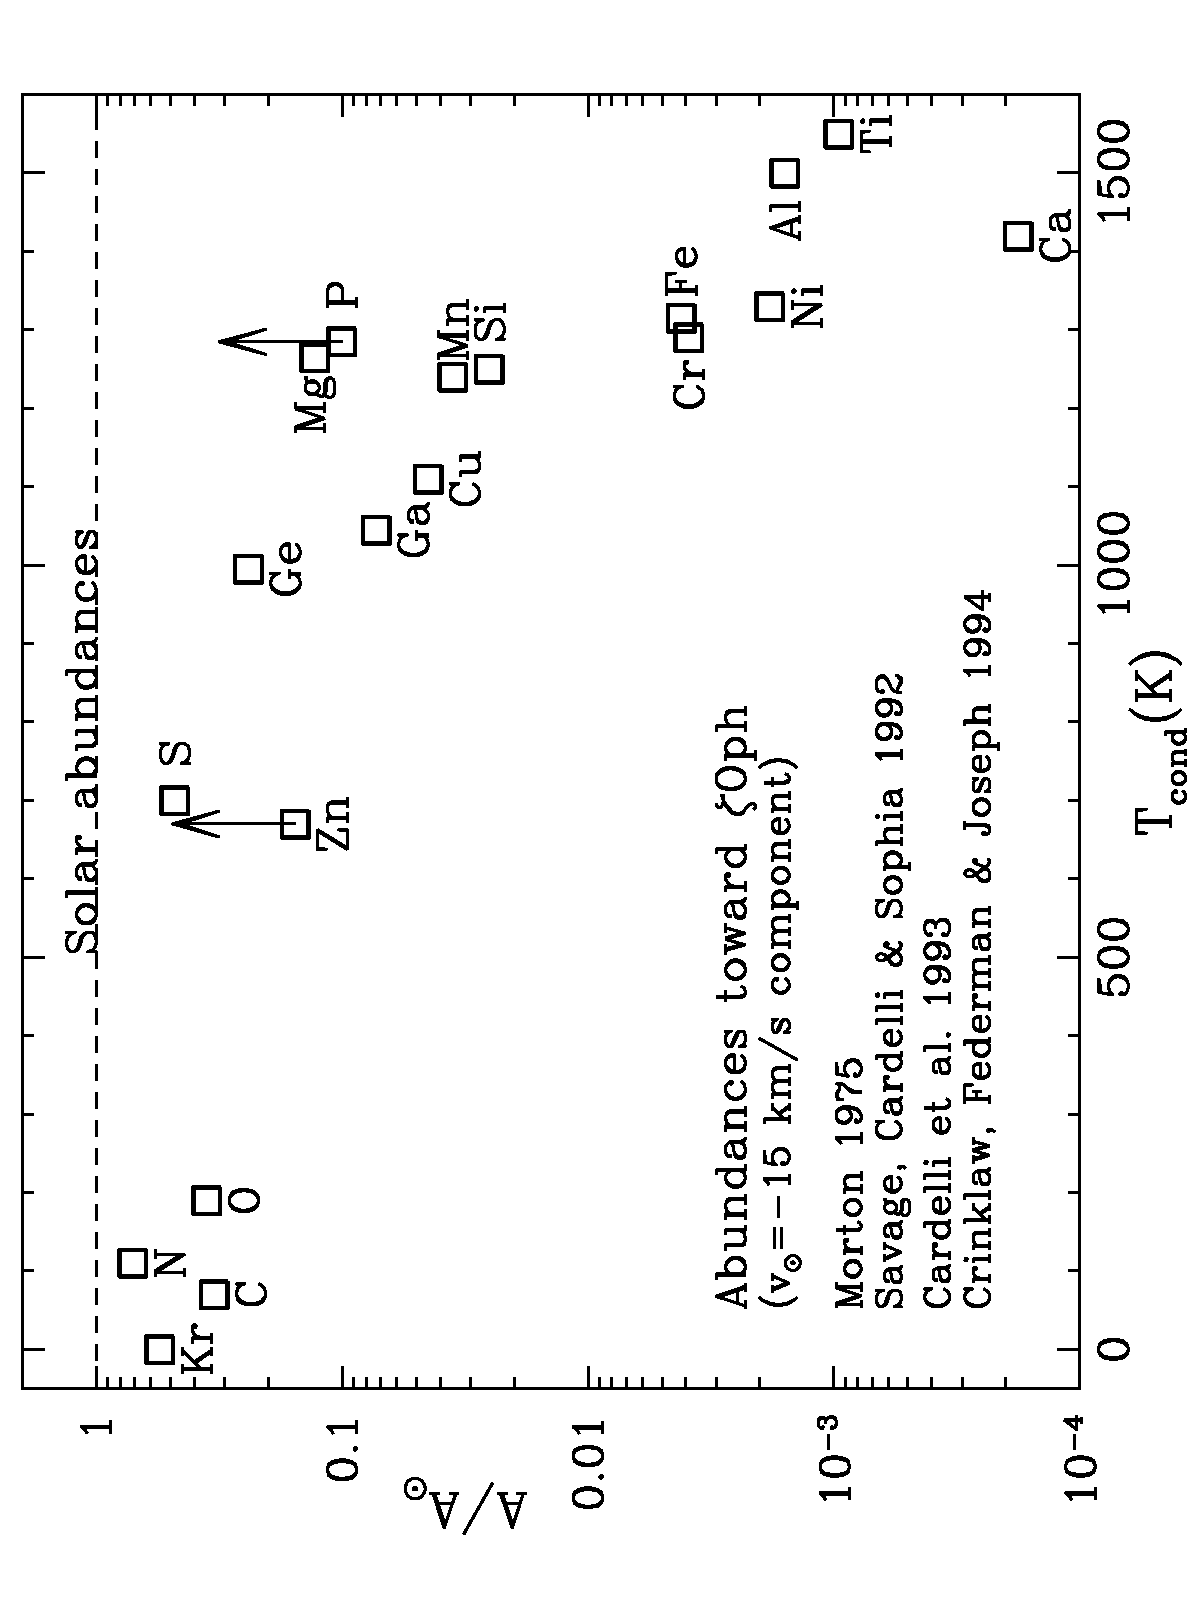
\includegraphics[width=\textwidth,height=!]{./A/zoph_depletion.pdf}}

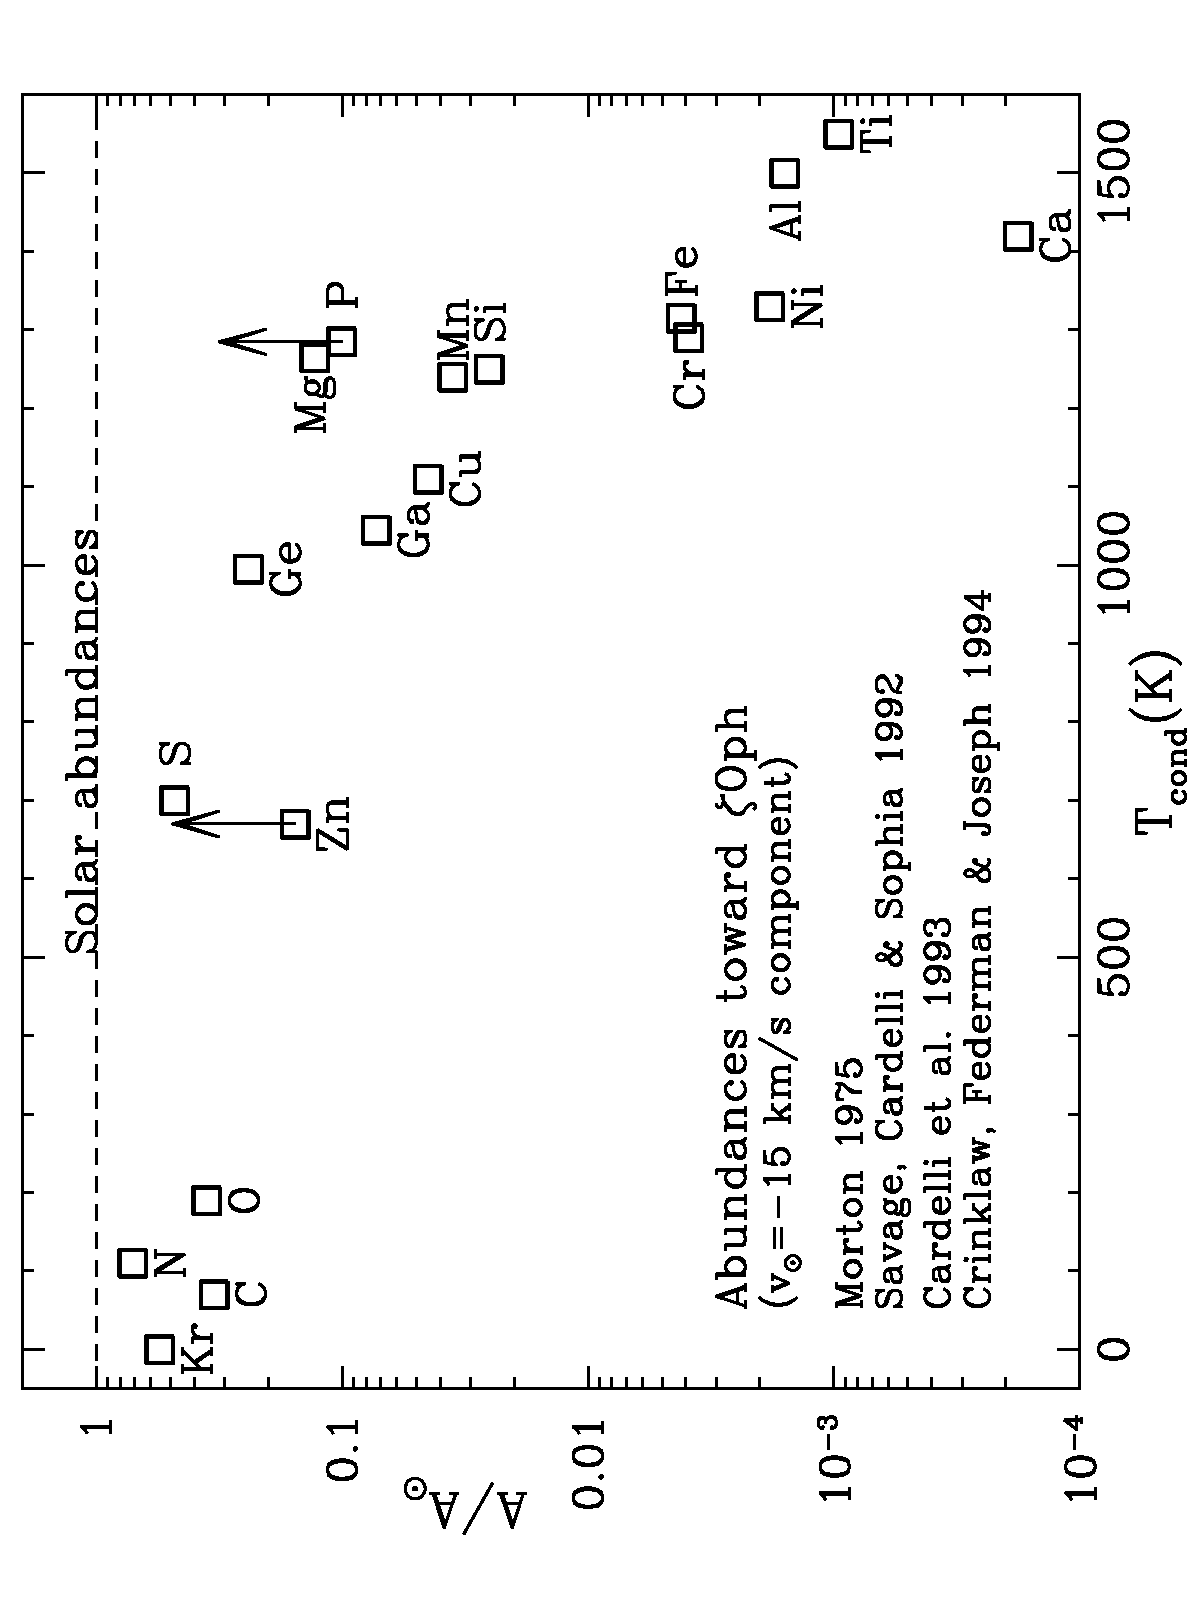
\includegraphics[width=0.7\textwidth,height=!,angle=-90]{./A/zoph_depletion.pdf}

  %{\tiny From \href{http://klab.agsci.colostate.edu/aegypti/aegypti.html}
  %{http://klab.agsci.colostate.edu/aegypti/aegypti.html}}
\end{center}
\end{columns}

}

\section{Mixing in the ISM}

\frame{  \frametitle{Mixing in the ISM} 

The isotopic ratio  $^{12}$C/$^{13}$C is a good tracer of the stellar
processing of the ISM. \medskip

\begin{columns}[t,onlytextwidth]

\column{0.5\textwidth}


\begin{center}
    \includegraphics[width=\textwidth,height=!]{./A/fig_ZOPH.pdf}

    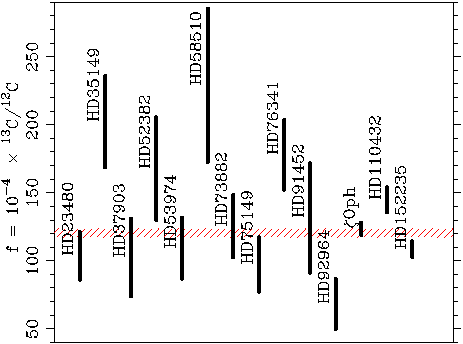
\includegraphics[width=0.6\textwidth,height=!]{./A/fig_all.pdf}
\end{center}


\column{0.5\textwidth}

  \begin{center}
    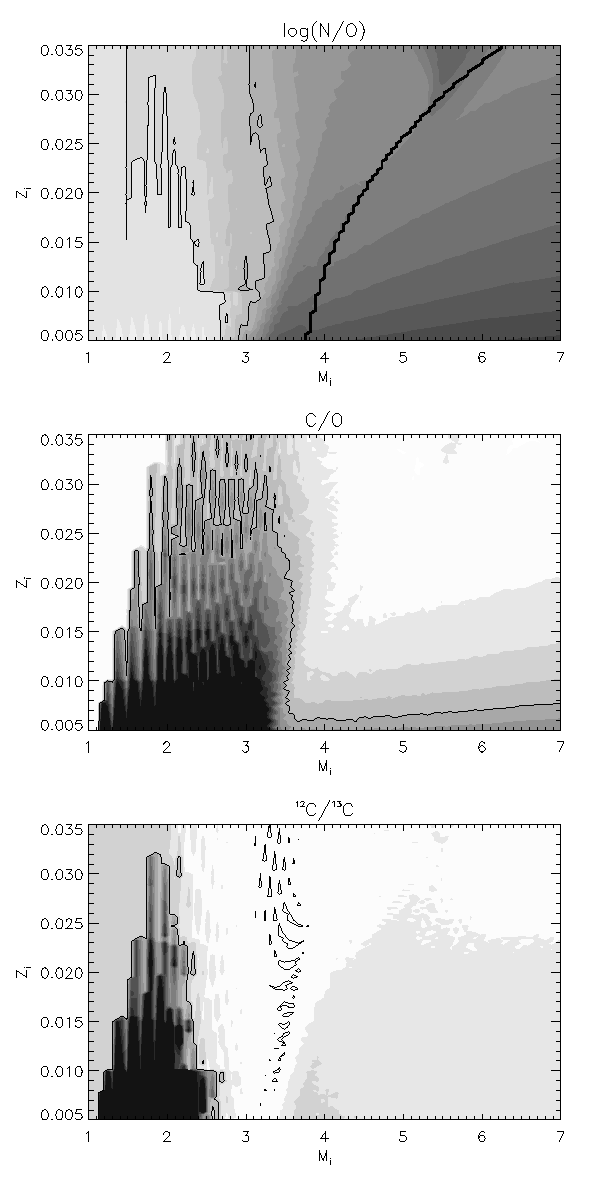
\includegraphics[width=0.7\textwidth,height=!]{./A/mz.pdf}   
  \end{center}
\end{columns}

}

\section{Emission mechanisms  in the  ISM}

\frame{ \frametitle{Emission mechanisms in the ISM - synchrotron}
{\tt http://lambda.gsfc.nasa.gov/product/map/} \\
\begin{center}
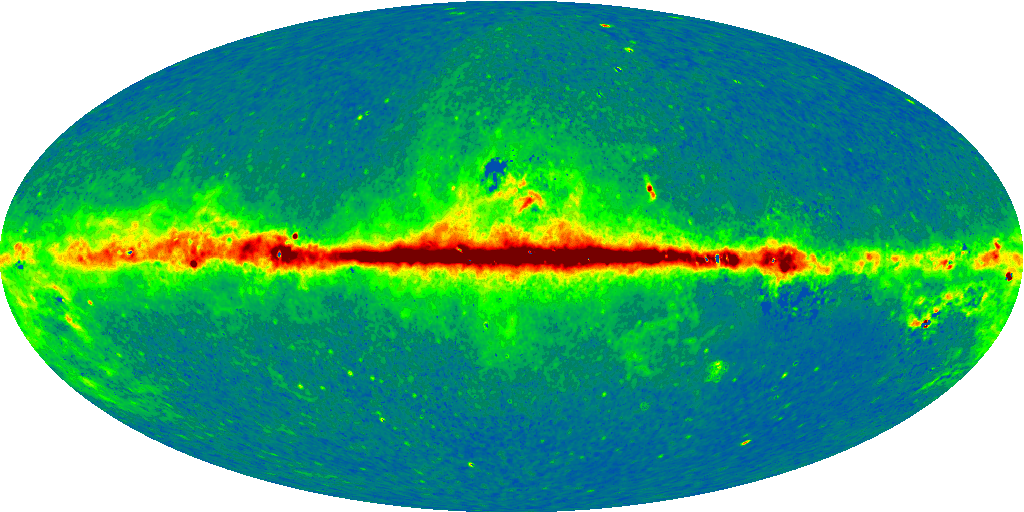
\includegraphics[width=\textwidth,height=!]{./A/lrg_mem_synch}
\end{center}
}

\frame{\frametitle{Emission mechanisms  - free-free}
\begin{center}
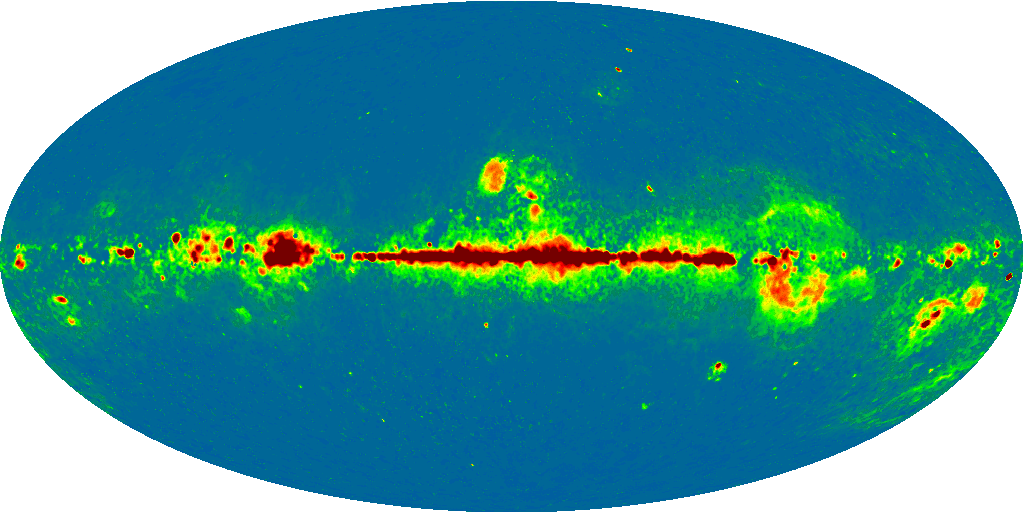
\includegraphics[width=\textwidth,height=!]{./A/lrg_mem_ff}
\end{center}
}

\frame{\frametitle{Emission mechanisms  - standard dust}
\begin{center}
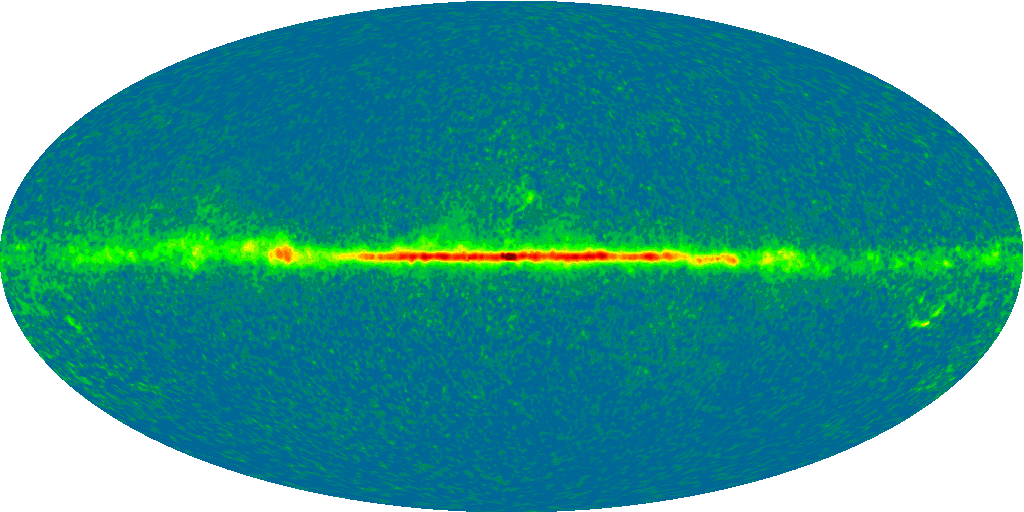
\includegraphics[width=\textwidth,height=!]{./A/lrg_mem_dust}
\end{center}
}

\frame{\frametitle{Conspicuous features}
\begin{center}
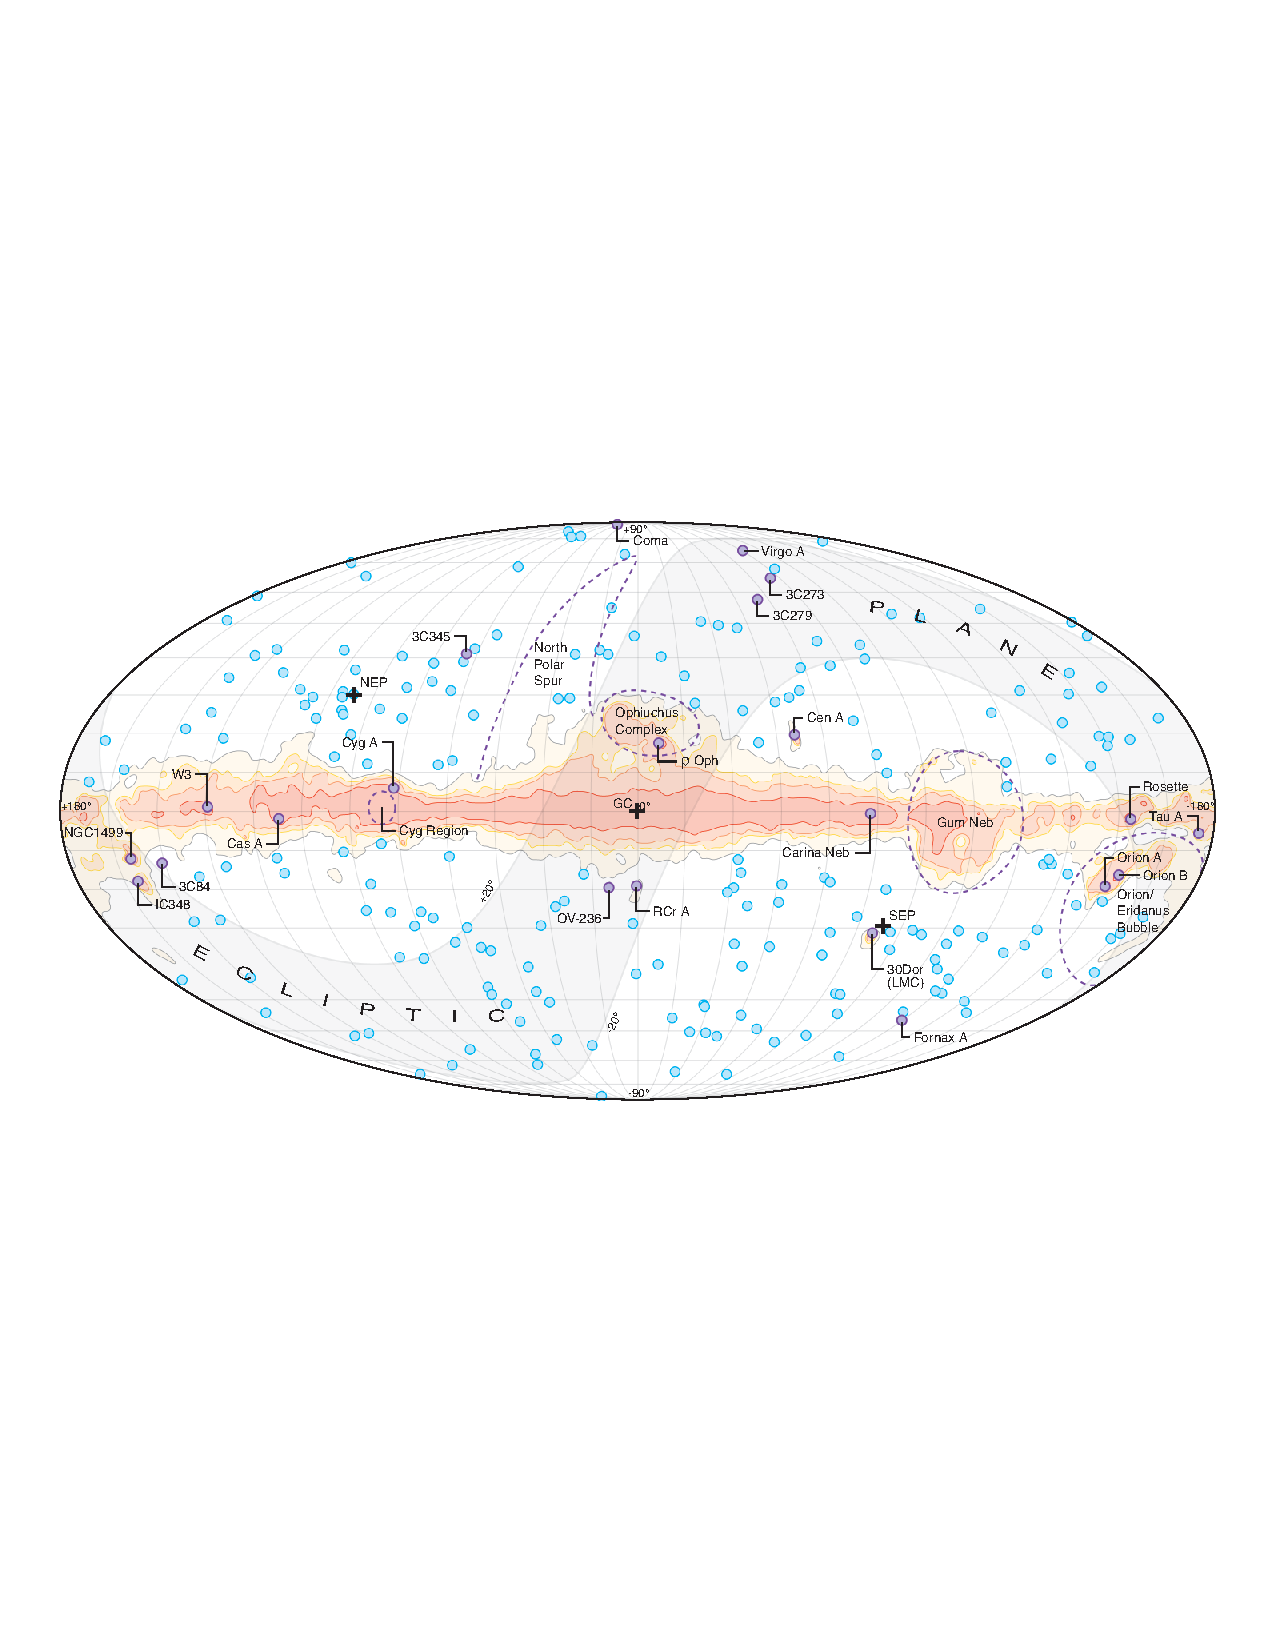
\includegraphics[width=\textwidth,height=!]{./A/wmap_expl}
\end{center}
}


\frame{ \frametitle{Conspicuous features - Planck} 

{\tt http://www.esa.int/SPECIALS/Planck/index.html}
\begin{center}
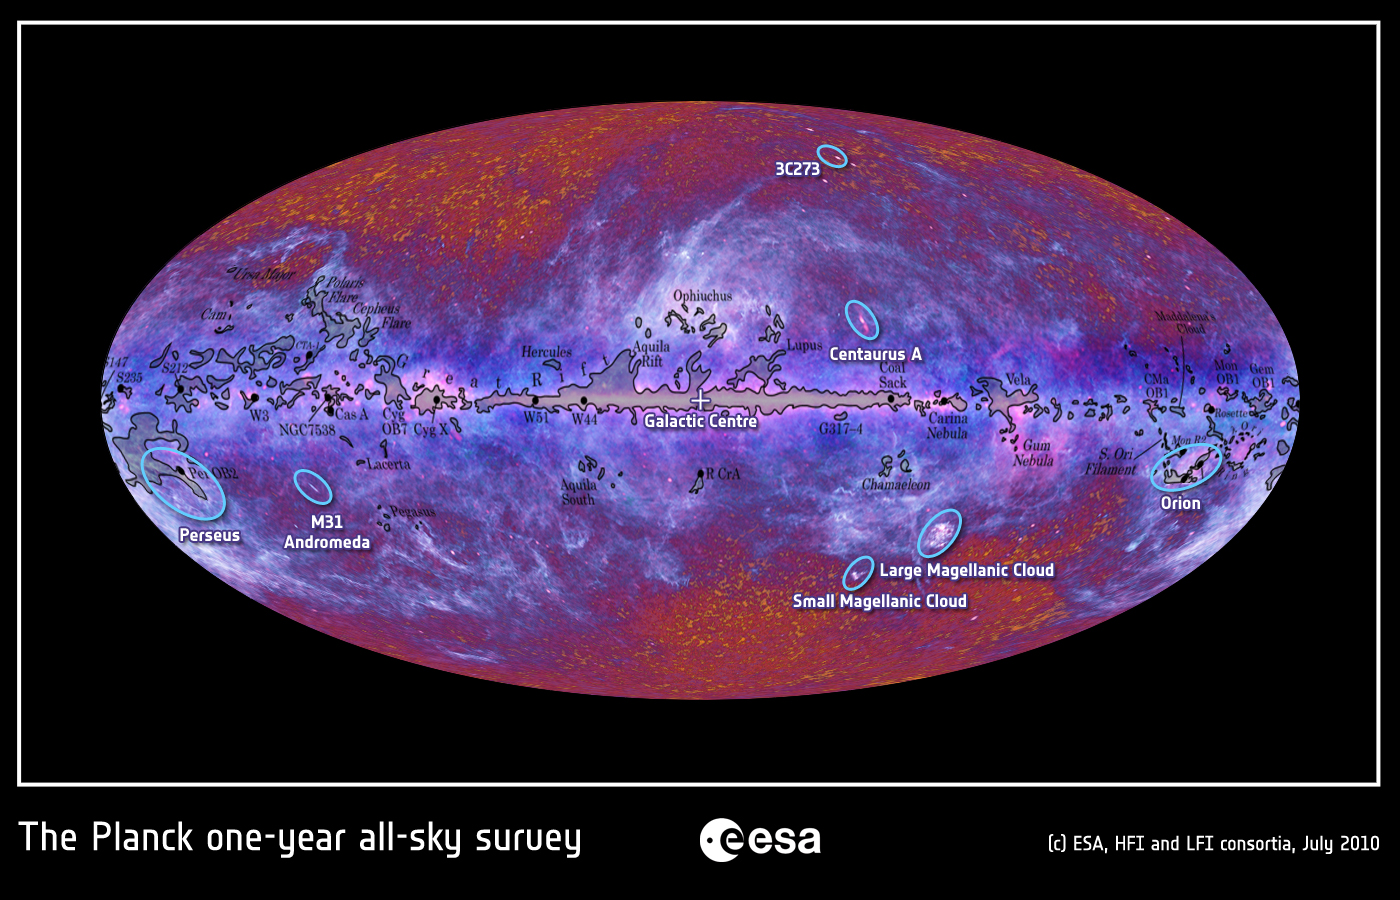
\includegraphics[width=\textwidth,height=!]{./A/PLANCK_FSM_03_Black_Regions_v02_B,0.jpg}
\end{center}
}

\frame{\frametitle{Example star forming region: Aquila Rift - Planck} 
\begin{center}
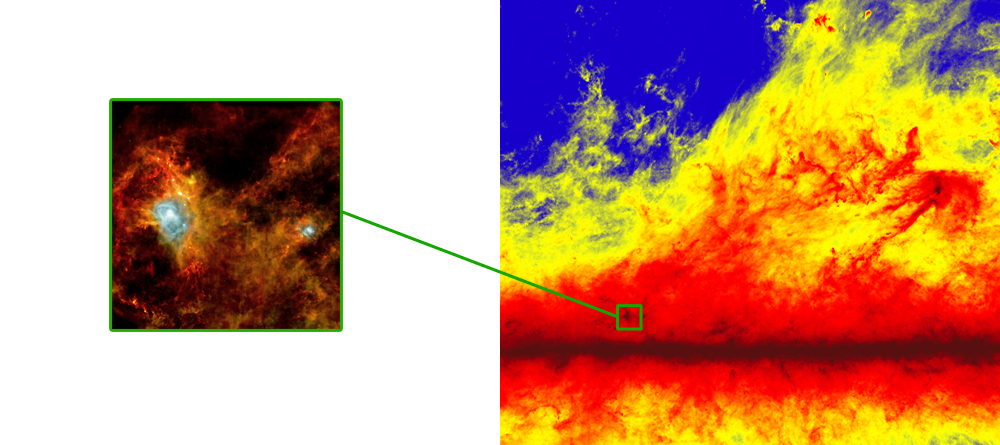
\includegraphics[width=\textwidth,height=!]{./A/P857_with_Aquila_white,2.jpg}
\end{center}
Left: Herschel, Right: Planck 
}

